% Investor prospectus "Risk Parity + Trend" -- Group Z, Financial Modeling (Nova SBE)
% Build: tectonic -X compile main.tex   (or VS Code + LaTeX Workshop, recipe "tectonic")
% Every result is printed with \res{key}; the values come from results_macros.tex, which the
% notebook (Section 10) writes. Do not type results by hand. Each value links to its notebook section.
\documentclass[10pt,a4paper]{article}

\usepackage{iftex}
\ifXeTeX
  \usepackage{fontspec}
  \setmainfont{texgyreheros}[Extension=.otf, UprightFont=*-regular, BoldFont=*-bold,
    ItalicFont=*-italic, BoldItalicFont=*-bolditalic]
\else
  \usepackage[T1]{fontenc}\usepackage[utf8]{inputenc}\usepackage{tgheros}\renewcommand{\familydefault}{\sfdefault}
\fi
\usepackage[a4paper,margin=1.9cm,top=1.7cm,bottom=1.8cm]{geometry}
\usepackage{amsmath}
\usepackage[table]{xcolor}
\usepackage{graphicx,booktabs,array,longtable,tabularx,multirow,float}
\usepackage[font=small,labelfont=bf,skip=3pt,position=top]{caption}
\usepackage[para,flushleft]{threeparttable}
\usepackage{enumitem}
\usepackage{multicol}
\usepackage{tcolorbox}
\usepackage[authoryear,round]{natbib}
\usepackage{fancyhdr}
\usepackage[colorlinks=true,linkcolor=black,citecolor=black,urlcolor=black]{hyperref}
% long URLs (app, repository) may also break at hyphens instead of running into the margin
\expandafter\def\expandafter\UrlBreaks\expandafter{\UrlBreaks\do\-}
\usepackage{resultref}

\definecolor{fmdark}{HTML}{0D366B}
\definecolor{fmlight}{HTML}{CDE2FB}
\definecolor{fmgrey}{HTML}{F0EFEC}
\setlength{\parindent}{0pt}
\setlength{\parskip}{4pt}
\setlist{nosep,leftmargin=1.2em}
\renewcommand{\arraystretch}{1.08}
\pagestyle{fancy}\fancyhf{}
\fancyhead[L]{\small\color{fmdark}Risk Parity + Trend --- Investor prospectus}
\fancyhead[R]{\small\color{fmdark}Group Z}
\fancyfoot[C]{\small\thepage}
\renewcommand{\headrulewidth}{0.4pt}
\newcommand{\sectionrule}{}
\makeatletter
\renewcommand\section{\@startsection{section}{1}{0pt}{8pt}{3pt}{\large\bfseries\color{fmdark}}}
\renewcommand\subsection{\@startsection{subsection}{2}{0pt}{5pt}{1pt}{\normalsize\bfseries\color{fmdark}}}
\makeatother

% AUTO-GENERATED by notebook/GroupZ_RiskParity_Trend.ipynb (Section 9). Do not edit.
% Data retrieved from Yahoo Finance via yfinance: 2026-11-22 10:49 UTC
% \defres{key}{value}{description}{notebook section}{link}{source}{retrieved}
\defres{data_retrieved}{2026-11-22 10:49 UTC}{Time stamp of the Yahoo Finance download}{\S1}{https://nbviewer.org/github/paul2108/04_Financial-Modelin-Group-projects/blob/main/notebook/GroupZ_RiskParity_Trend.ipynb\#sec-1}{YF: all 9 series}{2026-11-22}
\defres{data_start}{01 Jan 2006}{First day of daily data requested}{\S0.2}{https://nbviewer.org/github/paul2108/04_Financial-Modelin-Group-projects/blob/main/notebook/GroupZ_RiskParity_Trend.ipynb\#sec-0-2}{YF: all 9 series}{2026-11-22}
\defres{data_end}{30 Oct 2026}{Last trading day in the sample}{\S2}{https://nbviewer.org/github/paul2108/04_Financial-Modelin-Group-projects/blob/main/notebook/GroupZ_RiskParity_Trend.ipynb\#sec-2}{YF: all 9 series}{2026-11-22}
\defres{first_decision}{28 Feb 2007}{First rebalancing date (decision at the close)}{\S3}{https://nbviewer.org/github/paul2108/04_Financial-Modelin-Group-projects/blob/main/notebook/GroupZ_RiskParity_Trend.ipynb\#sec-3}{YF: 6 ETFs}{2026-11-22}
\defres{sample_start}{Mar 2007}{First month with a strategy return}{\S3}{https://nbviewer.org/github/paul2108/04_Financial-Modelin-Group-projects/blob/main/notebook/GroupZ_RiskParity_Trend.ipynb\#sec-3}{YF: 6 ETFs}{2026-11-22}
\defres{sample_end}{Oct 2026}{Last month with a strategy return}{\S3}{https://nbviewer.org/github/paul2108/04_Financial-Modelin-Group-projects/blob/main/notebook/GroupZ_RiskParity_Trend.ipynb\#sec-3}{YF: 6 ETFs}{2026-11-22}
\defres{sample_months}{236}{Number of monthly returns in the backtest}{\S3}{https://nbviewer.org/github/paul2108/04_Financial-Modelin-Group-projects/blob/main/notebook/GroupZ_RiskParity_Trend.ipynb\#sec-3}{YF: 6 ETFs}{2026-11-22}
\defres{sample_years}{19.7}{Length of the backtest in years}{\S3}{https://nbviewer.org/github/paul2108/04_Financial-Modelin-Group-projects/blob/main/notebook/GroupZ_RiskParity_Trend.ipynb\#sec-3}{YF: 6 ETFs}{2026-11-22}
\defres{rf_mean}{1.5\%}{Average T-bill rate p.a. over the backtest}{\S3}{https://nbviewer.org/github/paul2108/04_Financial-Modelin-Group-projects/blob/main/notebook/GroupZ_RiskParity_Trend.ipynb\#sec-3}{YF: \textasciicircum{}IRX}{2026-11-22}
\defres{current_date}{31 Oct 2026}{Date of the current allocation}{\S4.6}{https://nbviewer.org/github/paul2108/04_Financial-Modelin-Group-projects/blob/main/notebook/GroupZ_RiskParity_Trend.ipynb\#sec-4-6}{YF: 6 ETFs}{2026-11-22}
\defres{n_above_trend}{4}{Asset classes above their 10-month SMA (Oct 2026)}{\S4.6}{https://nbviewer.org/github/paul2108/04_Financial-Modelin-Group-projects/blob/main/notebook/GroupZ_RiskParity_Trend.ipynb\#sec-4-6}{YF: 6 ETFs}{2026-11-22}
\defres{current_cash}{46.3\%}{Current weight in T-bills (Oct 2026)}{\S4.6}{https://nbviewer.org/github/paul2108/04_Financial-Modelin-Group-projects/blob/main/notebook/GroupZ_RiskParity_Trend.ipynb\#sec-4-6}{YF: 6 ETFs}{2026-11-22}
\defres{current_erc_spy}{13.2\%}{Current risk-parity weight of SPY}{\S4.6}{https://nbviewer.org/github/paul2108/04_Financial-Modelin-Group-projects/blob/main/notebook/GroupZ_RiskParity_Trend.ipynb\#sec-4-6}{YF: 6 ETFs}{2026-11-22}
\defres{current_erc_efa}{9.3\%}{Current risk-parity weight of EFA}{\S4.6}{https://nbviewer.org/github/paul2108/04_Financial-Modelin-Group-projects/blob/main/notebook/GroupZ_RiskParity_Trend.ipynb\#sec-4-6}{YF: 6 ETFs}{2026-11-22}
\defres{current_erc_ief}{41.2\%}{Current risk-parity weight of IEF}{\S4.6}{https://nbviewer.org/github/paul2108/04_Financial-Modelin-Group-projects/blob/main/notebook/GroupZ_RiskParity_Trend.ipynb\#sec-4-6}{YF: 6 ETFs}{2026-11-22}
\defres{current_erc_vnq}{14.0\%}{Current risk-parity weight of VNQ}{\S4.6}{https://nbviewer.org/github/paul2108/04_Financial-Modelin-Group-projects/blob/main/notebook/GroupZ_RiskParity_Trend.ipynb\#sec-4-6}{YF: 6 ETFs}{2026-11-22}
\defres{current_erc_dbc}{17.1\%}{Current risk-parity weight of DBC}{\S4.6}{https://nbviewer.org/github/paul2108/04_Financial-Modelin-Group-projects/blob/main/notebook/GroupZ_RiskParity_Trend.ipynb\#sec-4-6}{YF: 6 ETFs}{2026-11-22}
\defres{current_erc_gld}{5.1\%}{Current risk-parity weight of GLD}{\S4.6}{https://nbviewer.org/github/paul2108/04_Financial-Modelin-Group-projects/blob/main/notebook/GroupZ_RiskParity_Trend.ipynb\#sec-4-6}{YF: 6 ETFs}{2026-11-22}
\defres{strat_ann_mean}{4.6\%}{Strategy (net): average return p.a.}{\S6.1}{https://nbviewer.org/github/paul2108/04_Financial-Modelin-Group-projects/blob/main/notebook/GroupZ_RiskParity_Trend.ipynb\#sec-6-1}{YF: 6 ETFs, \textasciicircum{}IRX}{2026-11-22}
\defres{b6040_ann_mean}{8.1\%}{60/40 benchmark: average return p.a.}{\S6.1}{https://nbviewer.org/github/paul2108/04_Financial-Modelin-Group-projects/blob/main/notebook/GroupZ_RiskParity_Trend.ipynb\#sec-6-1}{YF: SPY, AGG, \textasciicircum{}IRX}{2026-11-22}
\defres{mkt_ann_mean}{11.7\%}{S\&P 500 TR: average return p.a.}{\S6.1}{https://nbviewer.org/github/paul2108/04_Financial-Modelin-Group-projects/blob/main/notebook/GroupZ_RiskParity_Trend.ipynb\#sec-6-1}{YF: \textasciicircum{}SP500TR, \textasciicircum{}IRX}{2026-11-22}
\defres{strat_cagr}{4.6\%}{Strategy (net): CAGR}{\S6.1}{https://nbviewer.org/github/paul2108/04_Financial-Modelin-Group-projects/blob/main/notebook/GroupZ_RiskParity_Trend.ipynb\#sec-6-1}{YF: 6 ETFs, \textasciicircum{}IRX}{2026-11-22}
\defres{b6040_cagr}{7.9\%}{60/40 benchmark: CAGR}{\S6.1}{https://nbviewer.org/github/paul2108/04_Financial-Modelin-Group-projects/blob/main/notebook/GroupZ_RiskParity_Trend.ipynb\#sec-6-1}{YF: SPY, AGG, \textasciicircum{}IRX}{2026-11-22}
\defres{mkt_cagr}{11.0\%}{S\&P 500 TR: CAGR}{\S6.1}{https://nbviewer.org/github/paul2108/04_Financial-Modelin-Group-projects/blob/main/notebook/GroupZ_RiskParity_Trend.ipynb\#sec-6-1}{YF: \textasciicircum{}SP500TR, \textasciicircum{}IRX}{2026-11-22}
\defres{strat_ann_vol}{4.7\%}{Strategy (net): volatility p.a.}{\S6.1}{https://nbviewer.org/github/paul2108/04_Financial-Modelin-Group-projects/blob/main/notebook/GroupZ_RiskParity_Trend.ipynb\#sec-6-1}{YF: 6 ETFs, \textasciicircum{}IRX}{2026-11-22}
\defres{b6040_ann_vol}{9.9\%}{60/40 benchmark: volatility p.a.}{\S6.1}{https://nbviewer.org/github/paul2108/04_Financial-Modelin-Group-projects/blob/main/notebook/GroupZ_RiskParity_Trend.ipynb\#sec-6-1}{YF: SPY, AGG, \textasciicircum{}IRX}{2026-11-22}
\defres{mkt_ann_vol}{15.4\%}{S\&P 500 TR: volatility p.a.}{\S6.1}{https://nbviewer.org/github/paul2108/04_Financial-Modelin-Group-projects/blob/main/notebook/GroupZ_RiskParity_Trend.ipynb\#sec-6-1}{YF: \textasciicircum{}SP500TR, \textasciicircum{}IRX}{2026-11-22}
\defres{strat_sharpe}{0.66}{Strategy (net): Sharpe ratio}{\S6.1}{https://nbviewer.org/github/paul2108/04_Financial-Modelin-Group-projects/blob/main/notebook/GroupZ_RiskParity_Trend.ipynb\#sec-6-1}{YF: 6 ETFs, \textasciicircum{}IRX}{2026-11-22}
\defres{b6040_sharpe}{0.67}{60/40 benchmark: Sharpe ratio}{\S6.1}{https://nbviewer.org/github/paul2108/04_Financial-Modelin-Group-projects/blob/main/notebook/GroupZ_RiskParity_Trend.ipynb\#sec-6-1}{YF: SPY, AGG, \textasciicircum{}IRX}{2026-11-22}
\defres{mkt_sharpe}{0.66}{S\&P 500 TR: Sharpe ratio}{\S6.1}{https://nbviewer.org/github/paul2108/04_Financial-Modelin-Group-projects/blob/main/notebook/GroupZ_RiskParity_Trend.ipynb\#sec-6-1}{YF: \textasciicircum{}SP500TR, \textasciicircum{}IRX}{2026-11-22}
\defres{strat_max_dd}{$-$5.7\%}{Strategy (net): maximum drawdown}{\S6.1}{https://nbviewer.org/github/paul2108/04_Financial-Modelin-Group-projects/blob/main/notebook/GroupZ_RiskParity_Trend.ipynb\#sec-6-1}{YF: 6 ETFs, \textasciicircum{}IRX}{2026-11-22}
\defres{b6040_max_dd}{$-$32.3\%}{60/40 benchmark: maximum drawdown}{\S6.1}{https://nbviewer.org/github/paul2108/04_Financial-Modelin-Group-projects/blob/main/notebook/GroupZ_RiskParity_Trend.ipynb\#sec-6-1}{YF: SPY, AGG, \textasciicircum{}IRX}{2026-11-22}
\defres{mkt_max_dd}{$-$50.9\%}{S\&P 500 TR: maximum drawdown}{\S6.1}{https://nbviewer.org/github/paul2108/04_Financial-Modelin-Group-projects/blob/main/notebook/GroupZ_RiskParity_Trend.ipynb\#sec-6-1}{YF: \textasciicircum{}SP500TR, \textasciicircum{}IRX}{2026-11-22}
\defres{strat_worst_12m}{$-$5.7\%}{Strategy (net): worst 12-month return}{\S6.1}{https://nbviewer.org/github/paul2108/04_Financial-Modelin-Group-projects/blob/main/notebook/GroupZ_RiskParity_Trend.ipynb\#sec-6-1}{YF: 6 ETFs, \textasciicircum{}IRX}{2026-11-22}
\defres{b6040_worst_12m}{$-$27.7\%}{60/40 benchmark: worst 12-month return}{\S6.1}{https://nbviewer.org/github/paul2108/04_Financial-Modelin-Group-projects/blob/main/notebook/GroupZ_RiskParity_Trend.ipynb\#sec-6-1}{YF: SPY, AGG, \textasciicircum{}IRX}{2026-11-22}
\defres{mkt_worst_12m}{$-$43.3\%}{S\&P 500 TR: worst 12-month return}{\S6.1}{https://nbviewer.org/github/paul2108/04_Financial-Modelin-Group-projects/blob/main/notebook/GroupZ_RiskParity_Trend.ipynb\#sec-6-1}{YF: \textasciicircum{}SP500TR, \textasciicircum{}IRX}{2026-11-22}
\defres{strat_final_value}{2.42}{Strategy (net): final value of \$1}{\S6.1}{https://nbviewer.org/github/paul2108/04_Financial-Modelin-Group-projects/blob/main/notebook/GroupZ_RiskParity_Trend.ipynb\#sec-6-1}{YF: 6 ETFs, \textasciicircum{}IRX}{2026-11-22}
\defres{b6040_final_value}{4.47}{60/40 benchmark: final value of \$1}{\S6.1}{https://nbviewer.org/github/paul2108/04_Financial-Modelin-Group-projects/blob/main/notebook/GroupZ_RiskParity_Trend.ipynb\#sec-6-1}{YF: SPY, AGG, \textasciicircum{}IRX}{2026-11-22}
\defres{mkt_final_value}{7.82}{S\&P 500 TR: final value of \$1}{\S6.1}{https://nbviewer.org/github/paul2108/04_Financial-Modelin-Group-projects/blob/main/notebook/GroupZ_RiskParity_Trend.ipynb\#sec-6-1}{YF: \textasciicircum{}SP500TR, \textasciicircum{}IRX}{2026-11-22}
\defres{strat_gross_sharpe}{0.71}{Strategy (gross): Sharpe ratio}{\S6.1}{https://nbviewer.org/github/paul2108/04_Financial-Modelin-Group-projects/blob/main/notebook/GroupZ_RiskParity_Trend.ipynb\#sec-6-1}{YF: 6 ETFs, \textasciicircum{}IRX}{2026-11-22}
\defres{strat_gross_ann_mean}{4.8\%}{Strategy (gross): average return p.a.}{\S6.1}{https://nbviewer.org/github/paul2108/04_Financial-Modelin-Group-projects/blob/main/notebook/GroupZ_RiskParity_Trend.ipynb\#sec-6-1}{YF: 6 ETFs}{2026-11-22}
\defres{strat_beta_mkt}{0.10}{Strategy (net): beta vs S\&P 500 (not annualised)}{\S6.1}{https://nbviewer.org/github/paul2108/04_Financial-Modelin-Group-projects/blob/main/notebook/GroupZ_RiskParity_Trend.ipynb\#sec-6-1}{YF: 6 ETFs, \textasciicircum{}SP500TR, \textasciicircum{}IRX}{2026-11-22}
\defres{strat_alpha_mkt}{2.1\%}{Strategy (net): Jensen's alpha vs S\&P 500 p.a.}{\S6.1}{https://nbviewer.org/github/paul2108/04_Financial-Modelin-Group-projects/blob/main/notebook/GroupZ_RiskParity_Trend.ipynb\#sec-6-1}{YF: 6 ETFs, \textasciicircum{}SP500TR, \textasciicircum{}IRX}{2026-11-22}
\defres{strat_alpha_mkt_t}{2.10}{Strategy (net): Newey-West t-statistic of alpha vs S\&P 500}{\S6.1}{https://nbviewer.org/github/paul2108/04_Financial-Modelin-Group-projects/blob/main/notebook/GroupZ_RiskParity_Trend.ipynb\#sec-6-1}{YF: 6 ETFs, \textasciicircum{}SP500TR, \textasciicircum{}IRX}{2026-11-22}
\defres{strat_beta_bench}{0.19}{Strategy (net): beta vs 60/40 (not annualised)}{\S6.1}{https://nbviewer.org/github/paul2108/04_Financial-Modelin-Group-projects/blob/main/notebook/GroupZ_RiskParity_Trend.ipynb\#sec-6-1}{YF: 6 ETFs, AGG, \textasciicircum{}IRX}{2026-11-22}
\defres{strat_alpha_bench}{1.8\%}{Strategy (net): alpha vs 60/40 p.a.}{\S6.1}{https://nbviewer.org/github/paul2108/04_Financial-Modelin-Group-projects/blob/main/notebook/GroupZ_RiskParity_Trend.ipynb\#sec-6-1}{YF: 6 ETFs, AGG, \textasciicircum{}IRX}{2026-11-22}
\defres{strat_alpha_bench_t}{1.90}{Strategy (net): Newey-West t-statistic of alpha vs 60/40}{\S6.1}{https://nbviewer.org/github/paul2108/04_Financial-Modelin-Group-projects/blob/main/notebook/GroupZ_RiskParity_Trend.ipynb\#sec-6-1}{YF: 6 ETFs, AGG, \textasciicircum{}IRX}{2026-11-22}
\defres{strat_tracking_error}{9.0\%}{Strategy (net): tracking error vs 60/40 p.a.}{\S6.1}{https://nbviewer.org/github/paul2108/04_Financial-Modelin-Group-projects/blob/main/notebook/GroupZ_RiskParity_Trend.ipynb\#sec-6-1}{YF: 6 ETFs, AGG, \textasciicircum{}IRX}{2026-11-22}
\defres{strat_info_ratio}{$-$0.39}{Strategy (net): information ratio vs 60/40}{\S6.1}{https://nbviewer.org/github/paul2108/04_Financial-Modelin-Group-projects/blob/main/notebook/GroupZ_RiskParity_Trend.ipynb\#sec-6-1}{YF: 6 ETFs, AGG, \textasciicircum{}IRX}{2026-11-22}
\defres{strat_turnover}{215.7\%}{Strategy (net): turnover p.a. (share of portfolio value traded)}{\S6.1}{https://nbviewer.org/github/paul2108/04_Financial-Modelin-Group-projects/blob/main/notebook/GroupZ_RiskParity_Trend.ipynb\#sec-6-1}{YF: 6 ETFs, \textasciicircum{}IRX}{2026-11-22}
\defres{strat_avg_cash}{31.6\%}{Strategy: average T-bill weight}{\S6.1}{https://nbviewer.org/github/paul2108/04_Financial-Modelin-Group-projects/blob/main/notebook/GroupZ_RiskParity_Trend.ipynb\#sec-6-1}{YF: 6 ETFs}{2026-11-22}
\defres{b6040_beta_mkt}{0.63}{60/40: beta vs S\&P 500}{\S6.1}{https://nbviewer.org/github/paul2108/04_Financial-Modelin-Group-projects/blob/main/notebook/GroupZ_RiskParity_Trend.ipynb\#sec-6-1}{YF: SPY, AGG, \textasciicircum{}SP500TR}{2026-11-22}
\defres{b6040_turnover}{24.4\%}{60/40: turnover p.a.}{\S6.1}{https://nbviewer.org/github/paul2108/04_Financial-Modelin-Group-projects/blob/main/notebook/GroupZ_RiskParity_Trend.ipynb\#sec-6-1}{YF: SPY, AGG}{2026-11-22}
\defres{ercnt_sharpe}{0.55}{ERC (no trend): sharpe}{\S6.1}{https://nbviewer.org/github/paul2108/04_Financial-Modelin-Group-projects/blob/main/notebook/GroupZ_RiskParity_Trend.ipynb\#sec-6-1}{YF: 6 ETFs, \textasciicircum{}IRX}{2026-11-22}
\defres{ercnt_max_dd}{$-$16.0\%}{ERC (no trend): max dd}{\S6.1}{https://nbviewer.org/github/paul2108/04_Financial-Modelin-Group-projects/blob/main/notebook/GroupZ_RiskParity_Trend.ipynb\#sec-6-1}{YF: 6 ETFs, \textasciicircum{}IRX}{2026-11-22}
\defres{ercnt_ann_vol}{7.1\%}{ERC (no trend): ann vol}{\S6.1}{https://nbviewer.org/github/paul2108/04_Financial-Modelin-Group-projects/blob/main/notebook/GroupZ_RiskParity_Trend.ipynb\#sec-6-1}{YF: 6 ETFs, \textasciicircum{}IRX}{2026-11-22}
\defres{ercnt_cagr}{5.3\%}{ERC (no trend): cagr}{\S6.1}{https://nbviewer.org/github/paul2108/04_Financial-Modelin-Group-projects/blob/main/notebook/GroupZ_RiskParity_Trend.ipynb\#sec-6-1}{YF: 6 ETFs, \textasciicircum{}IRX}{2026-11-22}
\defres{ewnt_sharpe}{0.50}{1/N (no trend): sharpe}{\S6.1}{https://nbviewer.org/github/paul2108/04_Financial-Modelin-Group-projects/blob/main/notebook/GroupZ_RiskParity_Trend.ipynb\#sec-6-1}{YF: 6 ETFs, \textasciicircum{}IRX}{2026-11-22}
\defres{ewnt_max_dd}{$-$36.8\%}{1/N (no trend): max dd}{\S6.1}{https://nbviewer.org/github/paul2108/04_Financial-Modelin-Group-projects/blob/main/notebook/GroupZ_RiskParity_Trend.ipynb\#sec-6-1}{YF: 6 ETFs, \textasciicircum{}IRX}{2026-11-22}
\defres{ewnt_ann_vol}{11.3\%}{1/N (no trend): ann vol}{\S6.1}{https://nbviewer.org/github/paul2108/04_Financial-Modelin-Group-projects/blob/main/notebook/GroupZ_RiskParity_Trend.ipynb\#sec-6-1}{YF: 6 ETFs, \textasciicircum{}IRX}{2026-11-22}
\defres{ewnt_cagr}{6.7\%}{1/N (no trend): cagr}{\S6.1}{https://nbviewer.org/github/paul2108/04_Financial-Modelin-Group-projects/blob/main/notebook/GroupZ_RiskParity_Trend.ipynb\#sec-6-1}{YF: 6 ETFs, \textasciicircum{}IRX}{2026-11-22}
\defres{sharpe_diff_6040}{$-$0.01}{Sharpe ratio: strategy minus 60/40}{\S6.1}{https://nbviewer.org/github/paul2108/04_Financial-Modelin-Group-projects/blob/main/notebook/GroupZ_RiskParity_Trend.ipynb\#sec-6-1}{YF: 6 ETFs, AGG, \textasciicircum{}IRX}{2026-11-22}
\defres{vol_ratio_6040}{0.48}{Volatility of the strategy relative to 60/40}{\S6.1}{https://nbviewer.org/github/paul2108/04_Financial-Modelin-Group-projects/blob/main/notebook/GroupZ_RiskParity_Trend.ipynb\#sec-6-1}{YF: 6 ETFs, AGG}{2026-11-22}
\defres{dd_ratio_6040}{0.17}{Maximum drawdown of the strategy relative to 60/40}{\S6.1}{https://nbviewer.org/github/paul2108/04_Financial-Modelin-Group-projects/blob/main/notebook/GroupZ_RiskParity_Trend.ipynb\#sec-6-1}{YF: 6 ETFs, AGG}{2026-11-22}
\defres{beta_mkt_loss10}{1.0}{Expected strategy move (\%) if equities move 10\% (10 x beta)}{\S6.1}{https://nbviewer.org/github/paul2108/04_Financial-Modelin-Group-projects/blob/main/notebook/GroupZ_RiskParity_Trend.ipynb\#sec-6-1}{YF: 6 ETFs, \textasciicircum{}SP500TR}{2026-11-22}
\defres{sharpe_se}{0.25}{Approximate standard error of the annual Sharpe ratio}{\S6.1}{https://nbviewer.org/github/paul2108/04_Financial-Modelin-Group-projects/blob/main/notebook/GroupZ_RiskParity_Trend.ipynb\#sec-6-1}{YF: 6 ETFs}{2026-11-22}
\defres{tab_performance}{Table~\ref{tab:performance}}{Performance measures (Table)}{\S6.1}{https://nbviewer.org/github/paul2108/04_Financial-Modelin-Group-projects/blob/main/notebook/GroupZ_RiskParity_Trend.ipynb\#sec-6-1}{YF: all 9 series}{2026-11-22}
\defres{fig_cumulative}{Figure~\ref{fig:cumulative}}{Cumulative performance (Figure)}{\S6.2}{https://nbviewer.org/github/paul2108/04_Financial-Modelin-Group-projects/blob/main/notebook/GroupZ_RiskParity_Trend.ipynb\#sec-6-2}{YF: all 9 series}{2026-11-22}
\defres{fig_drawdowns}{Figure~\ref{fig:drawdowns}}{Drawdowns (Figure)}{\S6.3}{https://nbviewer.org/github/paul2108/04_Financial-Modelin-Group-projects/blob/main/notebook/GroupZ_RiskParity_Trend.ipynb\#sec-6-3}{YF: all 9 series}{2026-11-22}
\defres{strat_maxdd_date}{Jan 2016}{Strategy: month of the maximum drawdown}{\S6.3}{https://nbviewer.org/github/paul2108/04_Financial-Modelin-Group-projects/blob/main/notebook/GroupZ_RiskParity_Trend.ipynb\#sec-6-3}{YF: 6 ETFs}{2026-11-22}
\defres{b6040_maxdd_date}{Feb 2009}{60/40: month of the maximum drawdown}{\S6.3}{https://nbviewer.org/github/paul2108/04_Financial-Modelin-Group-projects/blob/main/notebook/GroupZ_RiskParity_Trend.ipynb\#sec-6-3}{YF: SPY, AGG, \textasciicircum{}SP500TR}{2026-11-22}
\defres{mkt_maxdd_date}{Feb 2009}{S\&P 500 TR: month of the maximum drawdown}{\S6.3}{https://nbviewer.org/github/paul2108/04_Financial-Modelin-Group-projects/blob/main/notebook/GroupZ_RiskParity_Trend.ipynb\#sec-6-3}{YF: SPY, AGG, \textasciicircum{}SP500TR}{2026-11-22}
\defres{fig_weights}{Figure~\ref{fig:weights}}{Target weights over time (Figure)}{\S6.4}{https://nbviewer.org/github/paul2108/04_Financial-Modelin-Group-projects/blob/main/notebook/GroupZ_RiskParity_Trend.ipynb\#sec-6-4}{YF: 6 ETFs}{2026-11-22}
\defres{avg_w_spy}{9.1\%}{Average target weight of SPY}{\S6.4}{https://nbviewer.org/github/paul2108/04_Financial-Modelin-Group-projects/blob/main/notebook/GroupZ_RiskParity_Trend.ipynb\#sec-6-4}{YF: 6 ETFs}{2026-11-22}
\defres{avg_w_efa}{6.4\%}{Average target weight of EFA}{\S6.4}{https://nbviewer.org/github/paul2108/04_Financial-Modelin-Group-projects/blob/main/notebook/GroupZ_RiskParity_Trend.ipynb\#sec-6-4}{YF: 6 ETFs}{2026-11-22}
\defres{avg_w_ief}{33.1\%}{Average target weight of IEF}{\S6.4}{https://nbviewer.org/github/paul2108/04_Financial-Modelin-Group-projects/blob/main/notebook/GroupZ_RiskParity_Trend.ipynb\#sec-6-4}{YF: 6 ETFs}{2026-11-22}
\defres{avg_w_vnq}{5.6\%}{Average target weight of VNQ}{\S6.4}{https://nbviewer.org/github/paul2108/04_Financial-Modelin-Group-projects/blob/main/notebook/GroupZ_RiskParity_Trend.ipynb\#sec-6-4}{YF: 6 ETFs}{2026-11-22}
\defres{avg_w_dbc}{6.2\%}{Average target weight of DBC}{\S6.4}{https://nbviewer.org/github/paul2108/04_Financial-Modelin-Group-projects/blob/main/notebook/GroupZ_RiskParity_Trend.ipynb\#sec-6-4}{YF: 6 ETFs}{2026-11-22}
\defres{avg_w_gld}{7.8\%}{Average target weight of GLD}{\S6.4}{https://nbviewer.org/github/paul2108/04_Financial-Modelin-Group-projects/blob/main/notebook/GroupZ_RiskParity_Trend.ipynb\#sec-6-4}{YF: 6 ETFs}{2026-11-22}
\defres{avg_w_cash}{31.7\%}{Average target weight of CASH}{\S6.4}{https://nbviewer.org/github/paul2108/04_Financial-Modelin-Group-projects/blob/main/notebook/GroupZ_RiskParity_Trend.ipynb\#sec-6-4}{YF: 6 ETFs}{2026-11-22}
\defres{share_cash_months}{81.4\%}{Share of months with a T-bill position}{\S6.4}{https://nbviewer.org/github/paul2108/04_Financial-Modelin-Group-projects/blob/main/notebook/GroupZ_RiskParity_Trend.ipynb\#sec-6-4}{YF: 6 ETFs}{2026-11-22}
\defres{max_cash}{100.0\%}{Highest T-bill weight in any month}{\S6.4}{https://nbviewer.org/github/paul2108/04_Financial-Modelin-Group-projects/blob/main/notebook/GroupZ_RiskParity_Trend.ipynb\#sec-6-4}{YF: 6 ETFs}{2026-11-22}
\defres{max_cash_date}{Aug 2015}{Month of the highest T-bill weight}{\S6.4}{https://nbviewer.org/github/paul2108/04_Financial-Modelin-Group-projects/blob/main/notebook/GroupZ_RiskParity_Trend.ipynb\#sec-6-4}{YF: 6 ETFs}{2026-11-22}
\defres{bond_share_avg}{33.1\%}{Average weight of Treasuries (IEF)}{\S6.4}{https://nbviewer.org/github/paul2108/04_Financial-Modelin-Group-projects/blob/main/notebook/GroupZ_RiskParity_Trend.ipynb\#sec-6-4}{YF: 6 ETFs}{2026-11-22}
\defres{strat_ret_2008}{9.3\%}{Strategy: return in calendar year 2008}{\S6.5}{https://nbviewer.org/github/paul2108/04_Financial-Modelin-Group-projects/blob/main/notebook/GroupZ_RiskParity_Trend.ipynb\#sec-6-5}{YF: 6 ETFs, \textasciicircum{}IRX}{2026-11-22}
\defres{b6040_ret_2008}{$-$21.1\%}{60/40: return in calendar year 2008}{\S6.5}{https://nbviewer.org/github/paul2108/04_Financial-Modelin-Group-projects/blob/main/notebook/GroupZ_RiskParity_Trend.ipynb\#sec-6-5}{YF: SPY, AGG, \textasciicircum{}SP500TR}{2026-11-22}
\defres{mkt_ret_2008}{$-$37.0\%}{S\&P 500 TR: return in calendar year 2008}{\S6.5}{https://nbviewer.org/github/paul2108/04_Financial-Modelin-Group-projects/blob/main/notebook/GroupZ_RiskParity_Trend.ipynb\#sec-6-5}{YF: SPY, AGG, \textasciicircum{}SP500TR}{2026-11-22}
\defres{strat_ret_2020}{4.8\%}{Strategy: return in calendar year 2020}{\S6.5}{https://nbviewer.org/github/paul2108/04_Financial-Modelin-Group-projects/blob/main/notebook/GroupZ_RiskParity_Trend.ipynb\#sec-6-5}{YF: 6 ETFs, \textasciicircum{}IRX}{2026-11-22}
\defres{b6040_ret_2020}{14.6\%}{60/40: return in calendar year 2020}{\S6.5}{https://nbviewer.org/github/paul2108/04_Financial-Modelin-Group-projects/blob/main/notebook/GroupZ_RiskParity_Trend.ipynb\#sec-6-5}{YF: SPY, AGG, \textasciicircum{}SP500TR}{2026-11-22}
\defres{mkt_ret_2020}{18.4\%}{S\&P 500 TR: return in calendar year 2020}{\S6.5}{https://nbviewer.org/github/paul2108/04_Financial-Modelin-Group-projects/blob/main/notebook/GroupZ_RiskParity_Trend.ipynb\#sec-6-5}{YF: SPY, AGG, \textasciicircum{}SP500TR}{2026-11-22}
\defres{strat_ret_2022}{$-$3.7\%}{Strategy: return in calendar year 2022}{\S6.5}{https://nbviewer.org/github/paul2108/04_Financial-Modelin-Group-projects/blob/main/notebook/GroupZ_RiskParity_Trend.ipynb\#sec-6-5}{YF: 6 ETFs, \textasciicircum{}IRX}{2026-11-22}
\defres{b6040_ret_2022}{$-$15.9\%}{60/40: return in calendar year 2022}{\S6.5}{https://nbviewer.org/github/paul2108/04_Financial-Modelin-Group-projects/blob/main/notebook/GroupZ_RiskParity_Trend.ipynb\#sec-6-5}{YF: SPY, AGG, \textasciicircum{}SP500TR}{2026-11-22}
\defres{mkt_ret_2022}{$-$18.1\%}{S\&P 500 TR: return in calendar year 2022}{\S6.5}{https://nbviewer.org/github/paul2108/04_Financial-Modelin-Group-projects/blob/main/notebook/GroupZ_RiskParity_Trend.ipynb\#sec-6-5}{YF: SPY, AGG, \textasciicircum{}SP500TR}{2026-11-22}
\defres{years_beating_6040}{6}{Calendar years in which the strategy beat 60/40}{\S6.5}{https://nbviewer.org/github/paul2108/04_Financial-Modelin-Group-projects/blob/main/notebook/GroupZ_RiskParity_Trend.ipynb\#sec-6-5}{YF: 6 ETFs, AGG}{2026-11-22}
\defres{n_years_cal}{20}{Calendar years (incl. partial 2007 and 2026)}{\S6.5}{https://nbviewer.org/github/paul2108/04_Financial-Modelin-Group-projects/blob/main/notebook/GroupZ_RiskParity_Trend.ipynb\#sec-6-5}{YF: 6 ETFs}{2026-11-22}
\defres{roll_beta_min}{0.04}{Lowest rolling 60-month beta}{\S6.5}{https://nbviewer.org/github/paul2108/04_Financial-Modelin-Group-projects/blob/main/notebook/GroupZ_RiskParity_Trend.ipynb\#sec-6-5}{YF: 6 ETFs, \textasciicircum{}SP500TR}{2026-11-22}
\defres{roll_beta_max}{0.19}{Highest rolling 60-month beta}{\S6.5}{https://nbviewer.org/github/paul2108/04_Financial-Modelin-Group-projects/blob/main/notebook/GroupZ_RiskParity_Trend.ipynb\#sec-6-5}{YF: 6 ETFs, \textasciicircum{}SP500TR}{2026-11-22}
\defres{spy_index_gap}{0.09\%}{Average return gap S\&P 500 TR minus SPY p.a.}{\S7}{https://nbviewer.org/github/paul2108/04_Financial-Modelin-Group-projects/blob/main/notebook/GroupZ_RiskParity_Trend.ipynb\#sec-7}{YF: SPY, \textasciicircum{}SP500TR}{2026-11-22}
\defres{cost_drag}{0.22\%}{Annual cost drag at 10 bps}{\S8.1}{https://nbviewer.org/github/paul2108/04_Financial-Modelin-Group-projects/blob/main/notebook/GroupZ_RiskParity_Trend.ipynb\#sec-8-1}{YF: 6 ETFs}{2026-11-22}
\defres{cost_bps}{10 bps}{Assumed trading cost per unit of turnover}{\S0.2}{https://nbviewer.org/github/paul2108/04_Financial-Modelin-Group-projects/blob/main/notebook/GroupZ_RiskParity_Trend.ipynb\#sec-0-2}{Model assumption}{--}
\defres{breakeven_bps}{8 bps}{Break-even cost at which Sharpe equals 60/40}{\S8.1}{https://nbviewer.org/github/paul2108/04_Financial-Modelin-Group-projects/blob/main/notebook/GroupZ_RiskParity_Trend.ipynb\#sec-8-1}{YF: 6 ETFs, AGG, \textasciicircum{}IRX}{2026-11-22}
\defres{sharpe_cost50}{0.47}{Strategy Sharpe ratio at 50 bps}{\S8.1}{https://nbviewer.org/github/paul2108/04_Financial-Modelin-Group-projects/blob/main/notebook/GroupZ_RiskParity_Trend.ipynb\#sec-8-1}{YF: 6 ETFs, \textasciicircum{}IRX}{2026-11-22}
\defres{cagr_cost50}{3.7\%}{Strategy CAGR at 50 bps}{\S8.1}{https://nbviewer.org/github/paul2108/04_Financial-Modelin-Group-projects/blob/main/notebook/GroupZ_RiskParity_Trend.ipynb\#sec-8-1}{YF: 6 ETFs}{2026-11-22}
\defres{strat_gfc}{9.2\%}{Strategy: return, Financial crisis (Nov 2007–Feb 2009)}{\S8.2}{https://nbviewer.org/github/paul2108/04_Financial-Modelin-Group-projects/blob/main/notebook/GroupZ_RiskParity_Trend.ipynb\#sec-8-2}{YF: 6 ETFs, \textasciicircum{}IRX}{2026-11-22}
\defres{b6040_gfc}{$-$32.3\%}{60/40: return, Financial crisis (Nov 2007–Feb 2009)}{\S8.2}{https://nbviewer.org/github/paul2108/04_Financial-Modelin-Group-projects/blob/main/notebook/GroupZ_RiskParity_Trend.ipynb\#sec-8-2}{YF: SPY, AGG, \textasciicircum{}SP500TR}{2026-11-22}
\defres{mkt_gfc}{$-$50.9\%}{S\&P 500 TR: return, Financial crisis (Nov 2007–Feb 2009)}{\S8.2}{https://nbviewer.org/github/paul2108/04_Financial-Modelin-Group-projects/blob/main/notebook/GroupZ_RiskParity_Trend.ipynb\#sec-8-2}{YF: SPY, AGG, \textasciicircum{}SP500TR}{2026-11-22}
\defres{strat_covid}{0.1\%}{Strategy: return, Covid crash (Feb 2020–Mar 2020)}{\S8.2}{https://nbviewer.org/github/paul2108/04_Financial-Modelin-Group-projects/blob/main/notebook/GroupZ_RiskParity_Trend.ipynb\#sec-8-2}{YF: 6 ETFs, \textasciicircum{}IRX}{2026-11-22}
\defres{b6040_covid}{$-$11.5\%}{60/40: return, Covid crash (Feb 2020–Mar 2020)}{\S8.2}{https://nbviewer.org/github/paul2108/04_Financial-Modelin-Group-projects/blob/main/notebook/GroupZ_RiskParity_Trend.ipynb\#sec-8-2}{YF: SPY, AGG, \textasciicircum{}SP500TR}{2026-11-22}
\defres{mkt_covid}{$-$19.6\%}{S\&P 500 TR: return, Covid crash (Feb 2020–Mar 2020)}{\S8.2}{https://nbviewer.org/github/paul2108/04_Financial-Modelin-Group-projects/blob/main/notebook/GroupZ_RiskParity_Trend.ipynb\#sec-8-2}{YF: SPY, AGG, \textasciicircum{}SP500TR}{2026-11-22}
\defres{strat_infl}{$-$3.4\%}{Strategy: return, Inflation and rate shock (Jan 2022–Oct 2022)}{\S8.2}{https://nbviewer.org/github/paul2108/04_Financial-Modelin-Group-projects/blob/main/notebook/GroupZ_RiskParity_Trend.ipynb\#sec-8-2}{YF: 6 ETFs, \textasciicircum{}IRX}{2026-11-22}
\defres{b6040_infl}{$-$16.6\%}{60/40: return, Inflation and rate shock (Jan 2022–Oct 2022)}{\S8.2}{https://nbviewer.org/github/paul2108/04_Financial-Modelin-Group-projects/blob/main/notebook/GroupZ_RiskParity_Trend.ipynb\#sec-8-2}{YF: SPY, AGG, \textasciicircum{}SP500TR}{2026-11-22}
\defres{mkt_infl}{$-$17.7\%}{S\&P 500 TR: return, Inflation and rate shock (Jan 2022–Oct 2022)}{\S8.2}{https://nbviewer.org/github/paul2108/04_Financial-Modelin-Group-projects/blob/main/notebook/GroupZ_RiskParity_Trend.ipynb\#sec-8-2}{YF: SPY, AGG, \textasciicircum{}SP500TR}{2026-11-22}
\defres{strat_recov}{33.6\%}{Strategy: return, Recovery (Jan 2023–Oct 2026)}{\S8.2}{https://nbviewer.org/github/paul2108/04_Financial-Modelin-Group-projects/blob/main/notebook/GroupZ_RiskParity_Trend.ipynb\#sec-8-2}{YF: 6 ETFs, \textasciicircum{}IRX}{2026-11-22}
\defres{b6040_recov}{64.0\%}{60/40: return, Recovery (Jan 2023–Oct 2026)}{\S8.2}{https://nbviewer.org/github/paul2108/04_Financial-Modelin-Group-projects/blob/main/notebook/GroupZ_RiskParity_Trend.ipynb\#sec-8-2}{YF: SPY, AGG, \textasciicircum{}SP500TR}{2026-11-22}
\defres{mkt_recov}{108.0\%}{S\&P 500 TR: return, Recovery (Jan 2023–Oct 2026)}{\S8.2}{https://nbviewer.org/github/paul2108/04_Financial-Modelin-Group-projects/blob/main/notebook/GroupZ_RiskParity_Trend.ipynb\#sec-8-2}{YF: SPY, AGG, \textasciicircum{}SP500TR}{2026-11-22}
\defres{fig_sensitivity}{Figure~\ref{fig:sensitivity}}{Parameter sensitivity of the Sharpe ratio (Figure)}{\S8.3}{https://nbviewer.org/github/paul2108/04_Financial-Modelin-Group-projects/blob/main/notebook/GroupZ_RiskParity_Trend.ipynb\#sec-8-3}{YF: 6 ETFs, \textasciicircum{}IRX}{2026-11-22}
\defres{heat_min}{0.61}{Lowest Sharpe ratio in the parameter grid}{\S8.3}{https://nbviewer.org/github/paul2108/04_Financial-Modelin-Group-projects/blob/main/notebook/GroupZ_RiskParity_Trend.ipynb\#sec-8-3}{YF: 6 ETFs}{2026-11-22}
\defres{heat_max}{0.81}{Highest Sharpe ratio in the parameter grid}{\S8.3}{https://nbviewer.org/github/paul2108/04_Financial-Modelin-Group-projects/blob/main/notebook/GroupZ_RiskParity_Trend.ipynb\#sec-8-3}{YF: 6 ETFs}{2026-11-22}
\defres{heat_n}{21}{Number of parameter combinations tested}{\S8.3}{https://nbviewer.org/github/paul2108/04_Financial-Modelin-Group-projects/blob/main/notebook/GroupZ_RiskParity_Trend.ipynb\#sec-8-3}{YF: 6 ETFs}{2026-11-22}
\defres{loo_sharpe_min}{0.53}{Lowest Sharpe ratio when one asset class is left out}{\S8.4}{https://nbviewer.org/github/paul2108/04_Financial-Modelin-Group-projects/blob/main/notebook/GroupZ_RiskParity_Trend.ipynb\#sec-8-4}{YF: 6 ETFs, \textasciicircum{}IRX}{2026-11-22}
\defres{loo_sharpe_max}{0.75}{Highest Sharpe ratio when one asset class is left out}{\S8.4}{https://nbviewer.org/github/paul2108/04_Financial-Modelin-Group-projects/blob/main/notebook/GroupZ_RiskParity_Trend.ipynb\#sec-8-4}{YF: 6 ETFs, \textasciicircum{}IRX}{2026-11-22}
\defres{loo_worst_asset}{SPY}{Asset class whose removal lowers the Sharpe ratio most}{\S8.4}{https://nbviewer.org/github/paul2108/04_Financial-Modelin-Group-projects/blob/main/notebook/GroupZ_RiskParity_Trend.ipynb\#sec-8-4}{YF: 6 ETFs}{2026-11-22}
\defres{loo_sharpe_nogold}{0.56}{Sharpe ratio without gold}{\S8.4}{https://nbviewer.org/github/paul2108/04_Financial-Modelin-Group-projects/blob/main/notebook/GroupZ_RiskParity_Trend.ipynb\#sec-8-4}{YF: 6 ETFs, \textasciicircum{}IRX}{2026-11-22}
\defres{loo_maxdd_worst}{$-$14.1\%}{Deepest drawdown when one asset class is left out}{\S8.4}{https://nbviewer.org/github/paul2108/04_Financial-Modelin-Group-projects/blob/main/notebook/GroupZ_RiskParity_Trend.ipynb\#sec-8-4}{YF: 6 ETFs}{2026-11-22}
\defres{tab_leave_one_out}{Table~\ref{tab:loo}}{Leave-one-out robustness (Table)}{\S8.4}{https://nbviewer.org/github/paul2108/04_Financial-Modelin-Group-projects/blob/main/notebook/GroupZ_RiskParity_Trend.ipynb\#sec-8-4}{YF: 6 ETFs, \textasciicircum{}IRX}{2026-11-22}
\defres{hmm_data_start}{Jan 1990}{First month of S\&P 500 data used to train the HMM}{\S9}{https://nbviewer.org/github/paul2108/04_Financial-Modelin-Group-projects/blob/main/notebook/GroupZ_RiskParity_Trend.ipynb\#sec-9}{YF: \textasciicircum{}SP500TR}{2026-11-22}
\defres{ml_riskoff_hmm}{37.1\%}{Share of months the HMM signals risk-off}{\S9.1}{https://nbviewer.org/github/paul2108/04_Financial-Modelin-Group-projects/blob/main/notebook/GroupZ_RiskParity_Trend.ipynb\#sec-9-1}{YF: \textasciicircum{}SP500TR}{2026-11-22}
\defres{ml_riskoff_vol}{20.7\%}{Share of months the volatility rule signals risk-off}{\S9.1}{https://nbviewer.org/github/paul2108/04_Financial-Modelin-Group-projects/blob/main/notebook/GroupZ_RiskParity_Trend.ipynb\#sec-9-1}{YF: \textasciicircum{}SP500TR}{2026-11-22}
\defres{fig_regimes}{Figure~\ref{fig:regimes}}{HMM regimes, walk-forward (Figure)}{\S9.1}{https://nbviewer.org/github/paul2108/04_Financial-Modelin-Group-projects/blob/main/notebook/GroupZ_RiskParity_Trend.ipynb\#sec-9-1}{YF: \textasciicircum{}SP500TR}{2026-11-22}
\defres{ml_a_sharpe}{0.66}{A: Trend (base): sharpe}{\S9.2}{https://nbviewer.org/github/paul2108/04_Financial-Modelin-Group-projects/blob/main/notebook/GroupZ_RiskParity_Trend.ipynb\#sec-9-2}{YF: 6 ETFs, \textasciicircum{}SP500TR, \textasciicircum{}IRX}{2026-11-22}
\defres{ml_a_max_dd}{$-$5.7\%}{A: Trend (base): max dd}{\S9.2}{https://nbviewer.org/github/paul2108/04_Financial-Modelin-Group-projects/blob/main/notebook/GroupZ_RiskParity_Trend.ipynb\#sec-9-2}{YF: 6 ETFs, \textasciicircum{}SP500TR, \textasciicircum{}IRX}{2026-11-22}
\defres{ml_a_cagr}{4.6\%}{A: Trend (base): cagr}{\S9.2}{https://nbviewer.org/github/paul2108/04_Financial-Modelin-Group-projects/blob/main/notebook/GroupZ_RiskParity_Trend.ipynb\#sec-9-2}{YF: 6 ETFs, \textasciicircum{}SP500TR, \textasciicircum{}IRX}{2026-11-22}
\defres{ml_a_ann_vol}{4.7\%}{A: Trend (base): ann vol}{\S9.2}{https://nbviewer.org/github/paul2108/04_Financial-Modelin-Group-projects/blob/main/notebook/GroupZ_RiskParity_Trend.ipynb\#sec-9-2}{YF: 6 ETFs, \textasciicircum{}SP500TR, \textasciicircum{}IRX}{2026-11-22}
\defres{ml_a_turnover}{215.7\%}{A: Trend (base): turnover}{\S9.2}{https://nbviewer.org/github/paul2108/04_Financial-Modelin-Group-projects/blob/main/notebook/GroupZ_RiskParity_Trend.ipynb\#sec-9-2}{YF: 6 ETFs, \textasciicircum{}SP500TR, \textasciicircum{}IRX}{2026-11-22}
\defres{ml_b_sharpe}{0.61}{B: Volatility rule: sharpe}{\S9.2}{https://nbviewer.org/github/paul2108/04_Financial-Modelin-Group-projects/blob/main/notebook/GroupZ_RiskParity_Trend.ipynb\#sec-9-2}{YF: 6 ETFs, \textasciicircum{}SP500TR, \textasciicircum{}IRX}{2026-11-22}
\defres{ml_b_max_dd}{$-$15.7\%}{B: Volatility rule: max dd}{\S9.2}{https://nbviewer.org/github/paul2108/04_Financial-Modelin-Group-projects/blob/main/notebook/GroupZ_RiskParity_Trend.ipynb\#sec-9-2}{YF: 6 ETFs, \textasciicircum{}SP500TR, \textasciicircum{}IRX}{2026-11-22}
\defres{ml_b_cagr}{5.3\%}{B: Volatility rule: cagr}{\S9.2}{https://nbviewer.org/github/paul2108/04_Financial-Modelin-Group-projects/blob/main/notebook/GroupZ_RiskParity_Trend.ipynb\#sec-9-2}{YF: 6 ETFs, \textasciicircum{}SP500TR, \textasciicircum{}IRX}{2026-11-22}
\defres{ml_b_ann_vol}{6.4\%}{B: Volatility rule: ann vol}{\S9.2}{https://nbviewer.org/github/paul2108/04_Financial-Modelin-Group-projects/blob/main/notebook/GroupZ_RiskParity_Trend.ipynb\#sec-9-2}{YF: 6 ETFs, \textasciicircum{}SP500TR, \textasciicircum{}IRX}{2026-11-22}
\defres{ml_b_turnover}{77.8\%}{B: Volatility rule: turnover}{\S9.2}{https://nbviewer.org/github/paul2108/04_Financial-Modelin-Group-projects/blob/main/notebook/GroupZ_RiskParity_Trend.ipynb\#sec-9-2}{YF: 6 ETFs, \textasciicircum{}SP500TR, \textasciicircum{}IRX}{2026-11-22}
\defres{ml_b_verdict}{fails}{B: Volatility rule: result of the pre-registered promotion gates}{\S9.2}{https://nbviewer.org/github/paul2108/04_Financial-Modelin-Group-projects/blob/main/notebook/GroupZ_RiskParity_Trend.ipynb\#sec-9-2}{YF: 6 ETFs, \textasciicircum{}SP500TR, \textasciicircum{}IRX}{2026-11-22}
\defres{ml_b_stresswins}{0}{B: Volatility rule: stress periods with a better return than A}{\S9.2}{https://nbviewer.org/github/paul2108/04_Financial-Modelin-Group-projects/blob/main/notebook/GroupZ_RiskParity_Trend.ipynb\#sec-9-2}{YF: 6 ETFs, \textasciicircum{}SP500TR}{2026-11-22}
\defres{ml_c_sharpe}{0.58}{C: HMM: sharpe}{\S9.2}{https://nbviewer.org/github/paul2108/04_Financial-Modelin-Group-projects/blob/main/notebook/GroupZ_RiskParity_Trend.ipynb\#sec-9-2}{YF: 6 ETFs, \textasciicircum{}SP500TR, \textasciicircum{}IRX}{2026-11-22}
\defres{ml_c_max_dd}{$-$12.2\%}{C: HMM: max dd}{\S9.2}{https://nbviewer.org/github/paul2108/04_Financial-Modelin-Group-projects/blob/main/notebook/GroupZ_RiskParity_Trend.ipynb\#sec-9-2}{YF: 6 ETFs, \textasciicircum{}SP500TR, \textasciicircum{}IRX}{2026-11-22}
\defres{ml_c_cagr}{4.9\%}{C: HMM: cagr}{\S9.2}{https://nbviewer.org/github/paul2108/04_Financial-Modelin-Group-projects/blob/main/notebook/GroupZ_RiskParity_Trend.ipynb\#sec-9-2}{YF: 6 ETFs, \textasciicircum{}SP500TR, \textasciicircum{}IRX}{2026-11-22}
\defres{ml_c_ann_vol}{6.0\%}{C: HMM: ann vol}{\S9.2}{https://nbviewer.org/github/paul2108/04_Financial-Modelin-Group-projects/blob/main/notebook/GroupZ_RiskParity_Trend.ipynb\#sec-9-2}{YF: 6 ETFs, \textasciicircum{}SP500TR, \textasciicircum{}IRX}{2026-11-22}
\defres{ml_c_turnover}{85.2\%}{C: HMM: turnover}{\S9.2}{https://nbviewer.org/github/paul2108/04_Financial-Modelin-Group-projects/blob/main/notebook/GroupZ_RiskParity_Trend.ipynb\#sec-9-2}{YF: 6 ETFs, \textasciicircum{}SP500TR, \textasciicircum{}IRX}{2026-11-22}
\defres{ml_c_verdict}{fails}{C: HMM: result of the pre-registered promotion gates}{\S9.2}{https://nbviewer.org/github/paul2108/04_Financial-Modelin-Group-projects/blob/main/notebook/GroupZ_RiskParity_Trend.ipynb\#sec-9-2}{YF: 6 ETFs, \textasciicircum{}SP500TR, \textasciicircum{}IRX}{2026-11-22}
\defres{ml_c_stresswins}{0}{C: HMM: stress periods with a better return than A}{\S9.2}{https://nbviewer.org/github/paul2108/04_Financial-Modelin-Group-projects/blob/main/notebook/GroupZ_RiskParity_Trend.ipynb\#sec-9-2}{YF: 6 ETFs, \textasciicircum{}SP500TR}{2026-11-22}
\defres{ml_d_sharpe}{0.61}{D: Trend + HMM: sharpe}{\S9.2}{https://nbviewer.org/github/paul2108/04_Financial-Modelin-Group-projects/blob/main/notebook/GroupZ_RiskParity_Trend.ipynb\#sec-9-2}{YF: 6 ETFs, \textasciicircum{}SP500TR, \textasciicircum{}IRX}{2026-11-22}
\defres{ml_d_max_dd}{$-$5.3\%}{D: Trend + HMM: max dd}{\S9.2}{https://nbviewer.org/github/paul2108/04_Financial-Modelin-Group-projects/blob/main/notebook/GroupZ_RiskParity_Trend.ipynb\#sec-9-2}{YF: 6 ETFs, \textasciicircum{}SP500TR, \textasciicircum{}IRX}{2026-11-22}
\defres{ml_d_cagr}{4.2\%}{D: Trend + HMM: cagr}{\S9.2}{https://nbviewer.org/github/paul2108/04_Financial-Modelin-Group-projects/blob/main/notebook/GroupZ_RiskParity_Trend.ipynb\#sec-9-2}{YF: 6 ETFs, \textasciicircum{}SP500TR, \textasciicircum{}IRX}{2026-11-22}
\defres{ml_d_ann_vol}{4.5\%}{D: Trend + HMM: ann vol}{\S9.2}{https://nbviewer.org/github/paul2108/04_Financial-Modelin-Group-projects/blob/main/notebook/GroupZ_RiskParity_Trend.ipynb\#sec-9-2}{YF: 6 ETFs, \textasciicircum{}SP500TR, \textasciicircum{}IRX}{2026-11-22}
\defres{ml_d_turnover}{226.5\%}{D: Trend + HMM: turnover}{\S9.2}{https://nbviewer.org/github/paul2108/04_Financial-Modelin-Group-projects/blob/main/notebook/GroupZ_RiskParity_Trend.ipynb\#sec-9-2}{YF: 6 ETFs, \textasciicircum{}SP500TR, \textasciicircum{}IRX}{2026-11-22}
\defres{ml_d_verdict}{fails}{D: Trend + HMM: result of the pre-registered promotion gates}{\S9.2}{https://nbviewer.org/github/paul2108/04_Financial-Modelin-Group-projects/blob/main/notebook/GroupZ_RiskParity_Trend.ipynb\#sec-9-2}{YF: 6 ETFs, \textasciicircum{}SP500TR, \textasciicircum{}IRX}{2026-11-22}
\defres{ml_d_stresswins}{2}{D: Trend + HMM: stress periods with a better return than A}{\S9.2}{https://nbviewer.org/github/paul2108/04_Financial-Modelin-Group-projects/blob/main/notebook/GroupZ_RiskParity_Trend.ipynb\#sec-9-2}{YF: 6 ETFs, \textasciicircum{}SP500TR}{2026-11-22}
\defres{tab_ml}{Table~\ref{tab:ml}}{Machine-learning variants (Table)}{\S9.2}{https://nbviewer.org/github/paul2108/04_Financial-Modelin-Group-projects/blob/main/notebook/GroupZ_RiskParity_Trend.ipynb\#sec-9-2}{YF: 6 ETFs, \textasciicircum{}SP500TR, \textasciicircum{}IRX}{2026-11-22}
\defres{ml_stress_threshold}{5\%}{Stress month: S\&P 500 falls by more than this in the next month}{\S9.3}{https://nbviewer.org/github/paul2108/04_Financial-Modelin-Group-projects/blob/main/notebook/GroupZ_RiskParity_Trend.ipynb\#sec-9-3}{YF: \textasciicircum{}SP500TR}{2026-11-22}
\defres{ml_n_stress}{24}{Stress months (S\&P 500 falls > 5\% next month)}{\S9.3}{https://nbviewer.org/github/paul2108/04_Financial-Modelin-Group-projects/blob/main/notebook/GroupZ_RiskParity_Trend.ipynb\#sec-9-3}{YF: \textasciicircum{}SP500TR}{2026-11-22}
\defres{ml_recall_trend}{45.8\%}{Trend (SPY below 10m SMA): share of stress months flagged}{\S9.3}{https://nbviewer.org/github/paul2108/04_Financial-Modelin-Group-projects/blob/main/notebook/GroupZ_RiskParity_Trend.ipynb\#sec-9-3}{YF: \textasciicircum{}SP500TR, SPY}{2026-11-22}
\defres{ml_precision_trend}{22.4\%}{Trend (SPY below 10m SMA): share of alarms followed by stress}{\S9.3}{https://nbviewer.org/github/paul2108/04_Financial-Modelin-Group-projects/blob/main/notebook/GroupZ_RiskParity_Trend.ipynb\#sec-9-3}{YF: \textasciicircum{}SP500TR, SPY}{2026-11-22}
\defres{ml_missed_trend}{13}{Trend (SPY below 10m SMA): missed stress months}{\S9.3}{https://nbviewer.org/github/paul2108/04_Financial-Modelin-Group-projects/blob/main/notebook/GroupZ_RiskParity_Trend.ipynb\#sec-9-3}{YF: \textasciicircum{}SP500TR, SPY}{2026-11-22}
\defres{ml_recall_vol}{45.8\%}{Volatility rule: share of stress months flagged}{\S9.3}{https://nbviewer.org/github/paul2108/04_Financial-Modelin-Group-projects/blob/main/notebook/GroupZ_RiskParity_Trend.ipynb\#sec-9-3}{YF: \textasciicircum{}SP500TR, SPY}{2026-11-22}
\defres{ml_precision_vol}{22.4\%}{Volatility rule: share of alarms followed by stress}{\S9.3}{https://nbviewer.org/github/paul2108/04_Financial-Modelin-Group-projects/blob/main/notebook/GroupZ_RiskParity_Trend.ipynb\#sec-9-3}{YF: \textasciicircum{}SP500TR, SPY}{2026-11-22}
\defres{ml_missed_vol}{13}{Volatility rule: missed stress months}{\S9.3}{https://nbviewer.org/github/paul2108/04_Financial-Modelin-Group-projects/blob/main/notebook/GroupZ_RiskParity_Trend.ipynb\#sec-9-3}{YF: \textasciicircum{}SP500TR, SPY}{2026-11-22}
\defres{ml_recall_hmm}{66.7\%}{HMM: share of stress months flagged}{\S9.3}{https://nbviewer.org/github/paul2108/04_Financial-Modelin-Group-projects/blob/main/notebook/GroupZ_RiskParity_Trend.ipynb\#sec-9-3}{YF: \textasciicircum{}SP500TR, SPY}{2026-11-22}
\defres{ml_precision_hmm}{18.2\%}{HMM: share of alarms followed by stress}{\S9.3}{https://nbviewer.org/github/paul2108/04_Financial-Modelin-Group-projects/blob/main/notebook/GroupZ_RiskParity_Trend.ipynb\#sec-9-3}{YF: \textasciicircum{}SP500TR, SPY}{2026-11-22}
\defres{ml_missed_hmm}{8}{HMM: missed stress months}{\S9.3}{https://nbviewer.org/github/paul2108/04_Financial-Modelin-Group-projects/blob/main/notebook/GroupZ_RiskParity_Trend.ipynb\#sec-9-3}{YF: \textasciicircum{}SP500TR, SPY}{2026-11-22}
\defres{ml_seed_min}{0.58}{Variant C: lowest Sharpe ratio over single seeds}{\S9.4}{https://nbviewer.org/github/paul2108/04_Financial-Modelin-Group-projects/blob/main/notebook/GroupZ_RiskParity_Trend.ipynb\#sec-9-4}{YF: 6 ETFs, \textasciicircum{}SP500TR, \textasciicircum{}IRX}{2026-11-22}
\defres{ml_seed_max}{0.58}{Variant C: highest Sharpe ratio over single seeds}{\S9.4}{https://nbviewer.org/github/paul2108/04_Financial-Modelin-Group-projects/blob/main/notebook/GroupZ_RiskParity_Trend.ipynb\#sec-9-4}{YF: 6 ETFs, \textasciicircum{}SP500TR, \textasciicircum{}IRX}{2026-11-22}
\defres{ml_3state_sharpe}{0.59}{Variant C with three HMM states: Sharpe ratio}{\S9.4}{https://nbviewer.org/github/paul2108/04_Financial-Modelin-Group-projects/blob/main/notebook/GroupZ_RiskParity_Trend.ipynb\#sec-9-4}{YF: 6 ETFs, \textasciicircum{}SP500TR, \textasciicircum{}IRX}{2026-11-22}

% No appendix (7-page limit): every value links straight to the notebook section that computes it
\makeatletter
\renewcommand{\res}[1]{\leavevmode\res@check{#1}\res@record{#1}\href{\csuse{res@url@#1}}{\csuse{res@val@#1}}}
\renewcommand{\resval}[3]{\leavevmode\res@check{#1}\res@check{#2}\href{\csuse{res@url@#1}}{#3}}
\robustify{\res}\robustify{\resval}
\makeatother
\newcommand{\appurl}{https://04financial-modelin-group-projects-u7jx8pavhcsfkqmkps5b5d.streamlit.app}
\newcommand{\repourl}{https://github.com/paul2108/04_Financial-Modelin-Group-projects}

\begin{document}

% ------------------------------------------------------------------ cover (not counted)
\begin{titlepage}
\thispagestyle{empty}
\vspace*{2.5cm}
{\color{fmdark}\rule{\linewidth}{1.2pt}}\\[8pt]
{\Huge\bfseries\color{fmdark} Risk Parity + Trend}\\[6pt]
{\Large A lower-drawdown alternative to the 60/40 portfolio}\\[4pt]
{\large Investor prospectus \textbullet{} Model portfolio of six asset-class ETFs}\\
{\color{fmdark}\rule{\linewidth}{1.2pt}}
\vspace{1.4cm}

\begin{tabular}{@{}ll@{}}
\textbf{Course} & Financial Modeling, Nova School of Business and Economics\\
\textbf{Moodle group} & Group Z\\[4pt]
\textbf{Members} & Gabriel Depraz (56900)\\
 & Marwan El-shazly (78218)\\
 & Bruno Francisco Barth (79727)\\
 & Tim Jonas Trompa (64287)\\
 & Paul Kuehl (64253)\\
 & Felix Schoenstein (80555)\\[4pt]
\textbf{Date} & 24 November 2026\\[4pt]
\textbf{Interactive app} & \href{\appurl}{\nolinkurl{04financial-modelin-group-projects-u7jx8pavhcsfkqmkps5b5d.streamlit.app}}\\
\textbf{Code \& notebook} & \href{\repourl}{\nolinkurl{github.com/paul2108/04_Financial-Modelin-Group-projects}}\\
\end{tabular}

\vfill
\small\textit{Past performance, in particular simulated past performance, is not a reliable indicator of future
results. This document was prepared for a university course and is not investment advice.}
\end{titlepage}
\setcounter{page}{1}

% ------------------------------------------------------------------ 1
\section{The strategy at a glance}
\begin{tcolorbox}[colback=fmgrey,colframe=fmdark,boxrule=0.6pt,arc=1pt,left=6pt,right=6pt,top=4pt,bottom=4pt]
\small
\begin{tabularx}{\linewidth}{@{}>{\bfseries}p{2.6cm}X@{}}
Objective & Equity-like participation with bond-like drawdowns: a rules-based alternative to 60/40 for cautious
investors who value avoiding deep losses over maximising return.\\
Holdings & Six liquid US-listed ETFs, one per asset class: US and developed ex-US equities, US Treasuries, real estate,
commodities and gold. Assets out of trend are held in T-bills.\\
Rule & Monthly: (1) weights that give each asset class the same share of portfolio risk (risk parity); (2) an asset is held
only above its 10-month average, otherwise its weight goes to T-bills.\\
Benchmark & 60/40: 60\% SPY (S\&P 500) and 40\% AGG (US aggregate bonds), rebalanced monthly, same costs.\\
Backtest & \res{sample_start}--\res{sample_end} (\res{sample_years} years), monthly, net of \res{cost_bps} per unit of turnover.\\
Key results & Volatility \res{strat_ann_vol} vs \res{b6040_ann_vol} (60/40) $\cdot$ maximum drawdown \res{strat_max_dd} vs
\res{b6040_max_dd} $\cdot$ Sharpe ratio \res{strat_sharpe} vs \res{b6040_sharpe} $\cdot$ average return \res{strat_ann_mean} vs
\res{b6040_ann_mean} p.a. $\cdot$ 2008: \res{strat_ret_2008} vs \res{b6040_ret_2008}.\\
ML check & A walk-forward hidden Markov model, Hierarchical Risk Parity and classifiers using HMM states and FinBERT tone
of FOMC statements failed pre-registered gates (classifier AUC \res{ext_auc_min}--\res{ext_auc_max}; Section~9). None of
the \res{imp_n_trials} variants tried was adopted.\\
Out of sample & On unused proxy data for \res{imp_oos_start}--\res{imp_oos_end} the rule again lost far less than 60/40
(maximum drawdown \res{imp_oos_a_maxdd} vs \res{imp_oos_6040_maxdd}; Section~8).\\
\end{tabularx}
\end{tcolorbox}
\vspace{-2pt}
\textbf{In one sentence:} over almost two decades the strategy matched the return per unit of risk of 60/40 with about half
its volatility and a fraction of its worst loss, but earned a clearly lower absolute return and lags in strong equity markets.
It is built for clients who would sell 60/40 in a crash, not for clients who want to beat it.


\section{Who the portfolio is for}
\textbf{Who it is for.} Wealth managers and private banks that advise \emph{cautious to balanced private clients},
typically aged 45--65, a few years before or at the start of retirement, with an investment horizon of about 7--10 years
over which they will start drawing on their savings. For these clients a deep loss is the main danger: once withdrawals
begin, assets are sold at low prices and the loss cannot be recovered by waiting (\emph{sequence-of-returns risk}). They
accept a lower return for a smoother path, still want growth above cash and inflation, and want a rule that their adviser
can explain on one page. The strategy is run in US dollars; euro-based clients use the UCITS funds and the currency hedge
of Section~7.

\textbf{Why not simply 60/40?} A 60/40 portfolio is the natural default for such clients, which is why it is our benchmark.
Its weakness is that equities dominate its risk: it lost \res{b6040_ret_2008} in 2008 and \res{b6040_ret_2022} in 2022,
exactly the kind of loss that makes a client sell at the bottom. The strategy is designed for clients who would abandon a
60/40 portfolio in such a crash.

\textbf{Why these six assets.} Each holding protects the client in a different economic scenario: US and international
equities and real estate grow when the economy expands, Treasuries gain in recessions, and commodities and gold hold their
value when inflation surprises. Nobody knows which scenario comes next, so the portfolio holds all of them, lets none of
them dominate its risk, and moves into T-bills when an asset class is in a sustained decline.

\textbf{Who should not buy it.} Clients who measure success against 60/40 or the stock market: the strategy beat 60/40 in
only \res{years_beating_6040} of \res{n_years_cal} calendar years and lags in long bull markets. Investors seeking maximum
long-term growth with a long horizon should hold more equities instead.


\section{What the portfolio holds}
The portfolio holds one large, liquid ETF per asset class (Table~\ref{tab:holdings}). The asset classes are those
of \citet{faber2007}, extended by gold, and were chosen for their economic role (Section~2), not because of their past
returns. Prices of the ETFs already reflect their fees.
% Static facts from issuer pages (not backtest results); sources: see \citet{issuers2026}.
\begin{table}[!htb]
\centering\footnotesize\setlength{\tabcolsep}{4pt}
\caption{Holdings, their role and their implementation for euro-based investors}\label{tab:holdings}
\begin{threeparttable}
\begin{tabularx}{\textwidth}{lllllX}
\toprule
\rowcolor{fmdark}\textcolor{white}{\textbf{ETF}} & \textcolor{white}{\textbf{Asset class}} & \textcolor{white}{\textbf{Role in the portfolio}} & \textcolor{white}{\textbf{Since}} & \textcolor{white}{\textbf{Fee}} & \textcolor{white}{\textbf{UCITS equivalent (TER)}}\\
SPY & US equities & growth engine & 1993 & 0.09\% & iShares Core S\&P 500, CSPX (0.07\%)\\
EFA & Dev.\ ex-US equities & int'l growth & 2001 & 0.32\% & Xtrackers MSCI World ex USA, EXUS (0.15\%)\\
IEF & US Treasuries 7--10y & recession hedge & 2002 & 0.15\% & iShares \$ Treasury 7--10yr, CSBGU0 (0.07\%)\\
VNQ & US real estate (REITs) & real assets, income & 2004 & 0.13\% & iShares US Property Yield, IUSP (0.40\%)\\
DBC & Broad commodities & inflation hedge & 2006 & 0.89\%$^a$ & iShares Div.\ Commodity Swap (0.19\%)\\
GLD & Gold & crisis hedge & 2004 & 0.40\% & iShares Physical Gold ETC, SGLN (0.12\%)\\
BIL & T-bills (cash) & safe asset & 2007 & 0.14\% & iShares \$ Treasury 0--1yr, IB01 (0.07\%)\\
\bottomrule
\end{tabularx}
\begin{tablenotes}\footnotesize
\item Fees: expense ratios from the issuers' product pages, accessed 20 Nov 2026 \citep{issuers2026}; $^a$ from a fund-data aggregator,
not confirmed on the issuer page. In the backtest the cash return is the T-bill yield (\texttt{\textasciicircum IRX}); BIL is the
investable proxy. UCITS funds are listed in Europe and are the vehicles EU retail investors can buy.
\end{tablenotes}
\end{threeparttable}
\end{table}

Over the whole backtest Treasuries (IEF) were the largest holding, with an average target weight of \res{avg_w_ief}; T-bills
averaged \res{strat_avg_cash} of the portfolio.


\section{How capital is allocated}
\textbf{Step 1 --- risk parity.} At each month-end $t$ we estimate the covariance matrix $\Sigma_t$ of the six ETFs from
the last 252 daily returns and choose weights $w$ so that every asset class contributes the same share of portfolio risk
\citep{maillard2010}:
\[
RC_i=\frac{w_i(\Sigma_t w)_i}{w^\top\Sigma_t w}=\frac{1}{6}\ \ \text{for all } i,\qquad w_i>0,\quad \textstyle\sum_i w_i=1 .
\]
There is no closed form, so the six equations are solved with SciPy's \texttt{fsolve}, following \citet{spinu2013}. In all
months the risk contributions are equal to within $10^{-8}$; the inverse-volatility fallback was never needed. Volatile
assets (equities, commodities) get small weights and stable ones (Treasuries) large weights, so no asset class dominates the
risk, as equities do in 60/40 \citep{asness2012}.

\textbf{Step 2 --- trend filter.} An asset class is held only if its month-end price is above its 10-month moving average
\citep{faber2007}; otherwise its weight goes to T-bills. Prices tend to trend over months \citep{moskowitz2012}, so the
filter exits asset classes in prolonged declines such as 2008 or the 2022 bond sell-off.

\textbf{Timing and rebalancing.} Weights are set with closing prices on the last trading day of month $t$ and earn the
returns of month $t+1$; no later information is used. Between monthly rebalancing dates holdings drift with prices.
\textbf{Motivation:} in our sample risk parity alone cut the drawdown of an equal-weighted portfolio from \res{ewnt_max_dd}
to \res{ercnt_max_dd}; the trend filter cut it further to \res{strat_max_dd} (Table~\ref{tab:performance}).


\section{Data and backtest assumptions}
\textbf{Source and sample.} Daily prices from Yahoo Finance, retrieved through the \texttt{yfinance} API for the six ETFs,
AGG, the S\&P 500 total return index (\texttt{\textasciicircum SP500TR}) and the 13-week T-bill yield (\texttt{\textasciicircum IRX}).
Data are requested from \res{data_start}; the last trading day is \res{data_end}. The youngest ETF (DBC, launched in February
2006) and the 252-day risk window set the first decision date to \res{first_decision}, so the backtest covers
\res{sample_months} monthly returns from \res{sample_start} to \res{sample_end}, including the global financial crisis, the
Covid crash and the 2022 rate shock.

\textbf{Adjustments and calculations.} Prices are adjusted for splits and distributions, so returns are total returns
after fund fees. Month-end values are the last close of each month; returns are simple returns, so that portfolio returns
are exact weighted sums. The cash return in month $t$ is the \texttt{\textasciicircum IRX} yield at the end of month $t-1$
divided by 12 (on average \res{rf_mean} p.a.). Trading costs of \res{cost_bps} are charged on turnover, the sum of the
absolute changes in the six ETF weights against their drifted weights, for the strategy and the benchmark alike; a switch
between an ETF and T-bills is therefore charged once. The performance measures are defined in the note to
Table~\ref{tab:performance} and explained for the client in Section~6. Every number in this prospectus is computed in the
notebook; clicking a value opens the notebook section that computes it.


\section{Historical performance}
\begin{figure}[!htb]
\centering
\caption{Growth of \$1 invested on \res{first_decision} (log scale), net of costs unless stated. The dashed line shows the
strategy before trading costs.}\label{fig:cumulative}
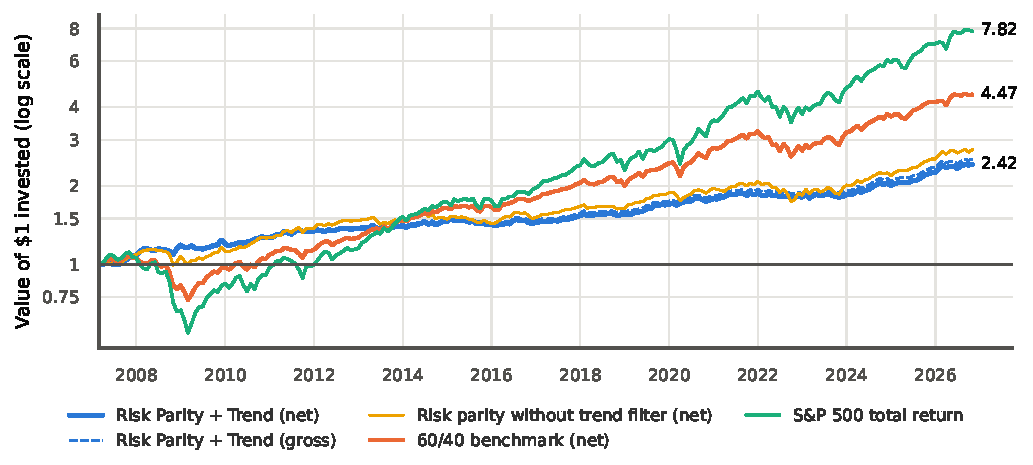
\includegraphics[width=\textwidth]{figures/fig_cumulative.pdf}\resmark{fig_cumulative}
\end{figure}

Figure~\ref{fig:cumulative} shows the central trade-off: \$1 grew to \$\res{strat_final_value} in the strategy,
\$\res{b6040_final_value} in 60/40 and \$\res{mkt_final_value} in the S\&P 500. The strategy led until 2014 because it avoided
the 2008 crash, then fell behind in the long bull market. Table~\ref{tab:performance} reports all measures.

\begin{table}[!htb]
\centering\small
\caption{Performance \res{sample_start}--\res{sample_end}, monthly returns, net of \res{cost_bps} per unit of turnover
(except ``Gross'')}\label{tab:performance}
\begin{threeparttable}
\begin{tabular}{@{}lrrrrrr@{}}
\toprule
\rowcolor{fmdark}\textcolor{white}{\textbf{Mar 2007--Oct 2026}} & \textcolor{white}{\textbf{Strategy}} & \textcolor{white}{\textbf{Gross}} & \textcolor{white}{\textbf{ERC}} & \textcolor{white}{\textbf{1/N}} & \textcolor{white}{\textbf{60/40}} & \textcolor{white}{\textbf{S\&P 500}} \\
\rowcolor{fmlight}\multicolumn{7}{@{}l}{\textbf{Return and risk}} \\
Average return (\% p.a.) & 4.6 & 4.8 & 5.4 & 7.1 & 8.1 & 11.7 \\
CAGR (\% p.a.) & 4.6 & 4.8 & 5.3 & 6.7 & 7.9 & 11.0 \\
Volatility (\% p.a.) & 4.7 & 4.7 & 7.1 & 11.3 & 9.9 & 15.4 \\
Sharpe ratio & 0.66 & 0.71 & 0.55 & 0.50 & 0.67 & 0.66 \\
Maximum drawdown (\%) & $-$5.7 & $-$5.4 & $-$16.0 & $-$36.8 & $-$32.3 & $-$50.9 \\
Worst 12 months (\%) & $-$5.7 & $-$5.4 & $-$13.4 & $-$34.2 & $-$27.7 & $-$43.3 \\
\rowcolor{fmlight}\multicolumn{7}{@{}l}{\textbf{Relative to the market (S\&P 500 TR)}} \\
Beta & 0.10 & 0.10 & 0.29 & 0.61 & 0.63 & 1.00 \\
Alpha (\% p.a.) & 2.1 & 2.3 & 0.9 & $-$0.6 & 0.2 & $-$0.0 \\
\quad $t$-stat (Newey-West) & 2.10 & 2.34 & 0.68 & $-$0.37 & 0.43 & -- \\
\rowcolor{fmlight}\multicolumn{7}{@{}l}{\textbf{Relative to the 60/40 benchmark}} \\
Beta & 0.19 & 0.19 & 0.53 & 0.98 & -- & 1.54 \\
Alpha (\% p.a.) & 1.8 & 2.0 & 0.4 & $-$0.9 & -- & 0.0 \\
\quad $t$-stat (Newey-West) & 1.90 & 2.14 & 0.35 & $-$0.58 & -- & 0.04 \\
Tracking error (\% p.a.) & 9.0 & 9.0 & 6.7 & 5.8 & -- & 6.0 \\
Information ratio & $-$0.39 & $-$0.36 & $-$0.41 & $-$0.18 & -- & 0.59 \\
\rowcolor{fmlight}\multicolumn{7}{@{}l}{\textbf{Implementation}} \\
Turnover (\% p.a.) & 215.7 & 215.7 & 51.1 & 37.5 & 24.4 & -- \\
Average T-bill weight (\%) & 31.6 & 31.6 & 0.0 & 0.0 & 0.0 & -- \\
Final value of \$1 & 2.42 & 2.52 & 2.75 & 3.55 & 4.47 & 7.82 \\
\bottomrule
\end{tabular}
\resmark{tab_performance}
\begin{tablenotes}\footnotesize
\item ERC = risk parity without trend filter; 1/N = equal weights without trend filter. Average return arithmetic $\times 12$;
volatility $\times\sqrt{12}$; Sharpe ratio on excess returns over T-bills; beta not annualised; alpha $\times 12$ (Jensen's
alpha); information ratio = annualised active return / tracking error. Turnover includes the initial purchase.
\end{tablenotes}
\end{threeparttable}
\end{table}

\textbf{What the measures mean for our client.}
\begin{itemize}[leftmargin=1em]
\item \emph{Average return} \res{strat_ann_mean} p.a. vs \res{b6040_ann_mean}: the client gives up about half of the 60/40
return, but still grows well above the T-bill rate of \res{rf_mean}.
\item \emph{Volatility} \res{strat_ann_vol} vs \res{b6040_ann_vol}: swings are about \res{vol_ratio_6040} times those of 60/40,
the risk of a short-to-medium bond fund rather than a balanced fund.
\item \emph{Sharpe ratio} \res{strat_sharpe} vs \res{b6040_sharpe}: the same reward per unit of risk; not a better portfolio, but a
\emph{less risky} one. With a standard error of about \res{sharpe_se} \citep{lo2002} the two are statistically indistinguishable.
\item \emph{Beta} \res{strat_beta_mkt} against the S\&P 500 (\res{strat_beta_bench} against 60/40): a 10\% equity fall implies a
loss of only about \res{beta_mkt_loss10}\%. The return hardly depends on the stock market.
\item \emph{Alpha} \res{strat_alpha_mkt} p.a. against the market ($t=\res{strat_alpha_mkt_t}$) and \res{strat_alpha_bench} against
60/40 ($t=\res{strat_alpha_bench_t}$): more than the CAPM predicts given the low market exposure. It is borderline significant
and mainly reflects Treasuries, gold and commodities, which a stock-market factor misses.
\item \emph{Information ratio} \res{strat_info_ratio} against 60/40, tracking error \res{strat_tracking_error}: the strategy
underperformed 60/40 and deviated from it a lot. Clients who judge success against 60/40 should not buy it; for our client
the drawdown matters.
\item \emph{Maximum drawdown} \res{strat_max_dd} vs \res{b6040_max_dd} (S\&P 500: \res{mkt_max_dd}): about a sixth of the 60/40
loss. Worst 12 months: \res{strat_worst_12m} vs \res{b6040_worst_12m}.
\item \emph{At equal risk:} levered monthly to a volatility target near that of 60/40 (realised \res{ext_lev10_ann_vol}; borrowing
slightly above the T-bill rate, before taxes), the strategy would have earned \res{ext_lev10_cagr} a year vs \res{b6040_cagr},
with a maximum drawdown of \res{ext_lev10_max_dd} vs \res{b6040_max_dd}. Capped at two times leverage, more realistic for private
clients, and borrowing at T-bills + 10 bps: \res{imp_lev_cap2_s10_cagr} a year (Sharpe ratio \res{imp_lev_cap2_s10_sharpe},
maximum drawdown \res{imp_lev_cap2_s10_maxdd}).
\end{itemize}

\begin{figure}[!htb]
\centering
\caption{Drawdown from the previous peak, net of costs.}\label{fig:drawdowns}
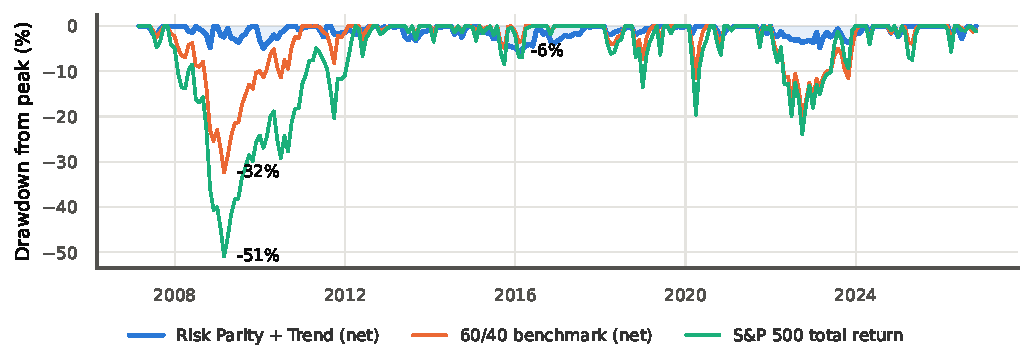
\includegraphics[width=\textwidth]{figures/fig_drawdowns.pdf}\resmark{fig_drawdowns}
\end{figure}

\textbf{Stress periods.} Financial crisis (Nov 2007--Feb 2009): strategy \res{strat_gfc}, 60/40 \res{b6040_gfc}; Covid crash
(Feb--Mar 2020): \res{strat_covid} vs \res{b6040_covid}; 2022 rate shock (Jan--Oct 2022): \res{strat_infl} vs \res{b6040_infl},
because the filter also sold Treasuries. The price is paid in recoveries: 2023--Oct 2026 \res{strat_recov} vs \res{b6040_recov}.
Figure~\ref{fig:weights} shows the shift into T-bills in falling markets.

\begin{figure}[!htb]
\centering
\caption{Target weights at each monthly rebalancing date. Grey: T-bills held because an asset class is below trend.}\label{fig:weights}
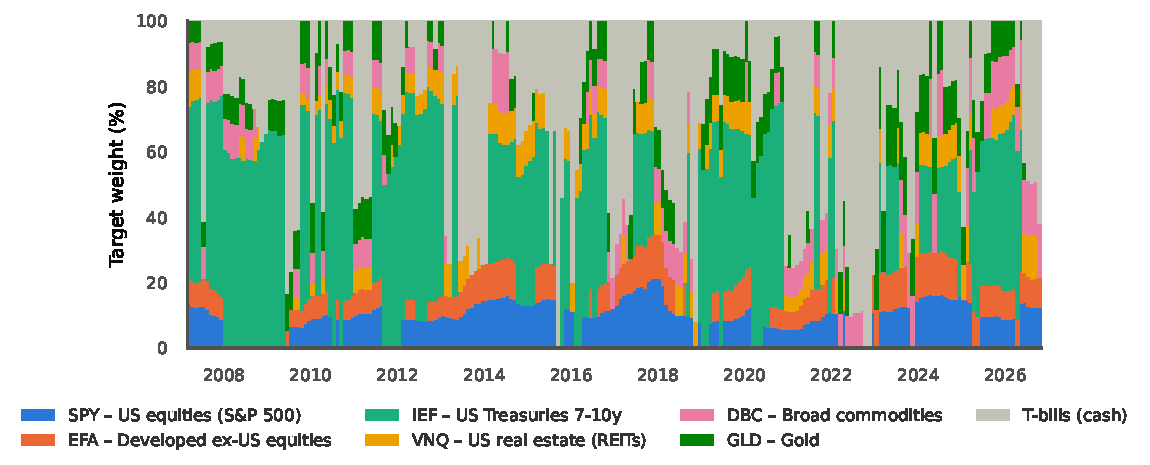
\includegraphics[width=\textwidth]{figures/fig_weights.pdf}\resmark{fig_weights}
\end{figure}


\section{Implementation and costs}
\textbf{Rebalancing.} Orders are placed once a month at the closing auction of the last trading day, using the weights computed
from that day's closing prices. All seven instruments (six ETFs and a T-bill ETF) trade billions of dollars a day, so a
portfolio of any realistic private-client size can be traded without moving prices. A model portfolio can be applied to
many client accounts at once.

\textbf{Turnover and costs.} The strategy trades \res{strat_turnover} of its value per year, against \res{b6040_turnover}
for 60/40: risk-parity weights change with volatility, and trend signals switch whole positions in and out. At our assumed
\res{cost_bps} per unit traded this costs \res{cost_drag} p.a.; the gross Sharpe ratio of \res{strat_gross_sharpe} falls to
\res{strat_sharpe} net. Solving $SR_{\text{strategy}}(c)=SR_{60/40}(c)$ with \texttt{fsolve} gives a \emph{break-even cost} of
\res{breakeven_bps}: above it, the 60/40 portfolio offers the better risk-adjusted return. Bid-ask spreads of these ETFs are
typically one basis point or less and commissions are often zero, so a cost-efficient platform is essential. At 50 bps the
Sharpe ratio would drop to \res{sharpe_cost50}. Simple ways to cut turnover are trading only weight changes above a threshold
and switching T-bill positions within a money-market sweep.

\textbf{Euro-based clients.} US-listed ETFs are not available to EU retail investors, so the UCITS equivalents in
Table~\ref{tab:holdings} are used. The backtest is in US dollars; a euro investor bears the EUR/USD exchange rate on the
whole portfolio. Because the strategy's own volatility is low, currency risk would dominate, so the bond and cash sleeves
should be held in EUR-hedged share classes. US investors should note that DBC issues a Schedule K-1 tax form; the
no-K-1 version (PDBC) tracks a similar index.


\section{Risks and limitations}
\begin{itemize}[leftmargin=1em]
\item \textbf{Concentration in interest-rate risk.} Treasuries are the least volatile asset and therefore receive the largest
weight (on average \res{avg_w_ief}). A simultaneous fall of bonds and equities, as in 2022, hits risk parity directly; the trend
filter limited the 2022 loss to \res{strat_ret_2022} but cannot prevent sudden shocks. Adding inflation-linked Treasuries
(TIP) as a seventh asset class hardly helped in the 2022 rate shock (\res{imp_tip_2022} vs \res{strat_infl}) and was not adopted.
\item \textbf{Trend reversals.} After a sharp fall and quick rebound the filter sells late and buys back late. In 2020 the
strategy returned \res{strat_ret_2020} while 60/40 earned \res{b6040_ret_2020}. In strong bull markets the client will often
lag: the strategy beat 60/40 in only \res{years_beating_6040} of \res{n_years_cal} calendar years.
\item \textbf{Look-ahead bias.} Every weight uses only prices up to its decision date; the truncation test of Section~4
confirms this.
\item \textbf{Survivorship and hindsight bias.} We hold broad asset classes instead of picked winners, and their ETFs are
among the largest of their kind. Still, the universe is chosen today. Leaving out any one asset class gives Sharpe ratios
between \res{loo_sharpe_min} and \res{loo_sharpe_max} (worst without \res{loo_worst_asset}; without gold \res{loo_sharpe_nogold})
and a maximum drawdown no worse than \res{loo_maxdd_worst}, so no single holding drives the result.
\item \textbf{Data snooping.} The 10-month average and the one-year risk window are fixed in advance from the literature. Across
all \res{heat_n} combinations of 6--12 months and 3, 6 or 12 months of risk data, the Sharpe ratio stays between \res{heat_min}
and \res{heat_max} (Figure~\ref{fig:sensitivity}): a plateau, not a lucky spike. Because trying many variants makes a good backtest easy to find by
chance \citep{bailey2014pbo}, the machine-learning variants of Section~9 were judged by gates fixed before the first run, so
they could not be tuned towards a better backtest; none of them was adopted.
\item \textbf{Statistical confidence.} In a circular block bootstrap \citep{politis1992} of several thousand resampled histories
(12-month blocks) the strategy's maximum drawdown is smaller than that of 60/40 in \res{ext_boot_p_mdd} of draws, while
its Sharpe ratio is higher in only \res{ext_boot_p_sharpe}: the lower drawdown is robust, the risk-adjusted return is the
same. The Sharpe ratio is similar in both halves of the sample (\res{ext_sub1_sharpe_a} and \res{ext_sub2_sharpe_a}).
\item \textbf{Rebalancing day.} Month-end was the most favourable of four tested rebalancing days. Rebalancing 0, 5, 10 or
15 trading days before month-end gives Sharpe ratios between \res{ext_offset_sharpe_min} and \res{ext_offset_sharpe_max}
and drawdowns of up to \res{ext_offset_mdd_worst}, still far smaller than those of 60/40. Four tranches with these rebalancing
days give \res{imp_m_sharpe}, close to their average; this is the more realistic expectation than the month-end result.
\item \textbf{Out-of-sample test.} As a final check we ran the rule on \res{imp_oos_start}--\res{imp_oos_end}, before the ETFs
existed, with long-history index funds as proxies. No free gold series exists for that period, so five of the six asset
classes are covered. The project had never used these data. The rule had a Sharpe ratio of \res{imp_oos_a_sharpe} and a
maximum drawdown of \res{imp_oos_a_maxdd}, against \res{imp_oos_6040_sharpe} and \res{imp_oos_6040_maxdd} for 60/40. Counting all
\res{imp_n_trials} variants tried in the notebook, the deflated Sharpe ratio \citep{bailey2014} still puts the probability that
the true Sharpe ratio is positive at \res{imp_dsr_a}.
\item \textbf{Short sample, model and data risk.} \res{sample_years} years contain only three major crises; the strategy's
results depend on how future crises unfold. Covariances are estimated with error, Yahoo Finance revises adjusted prices
occasionally, and the backtest assumes trading at closing prices without taxes.
\end{itemize}
\begin{figure}[!htb]
\centering
\caption{Net Sharpe ratio for different trend and risk windows; * marks the base case.}\label{fig:sensitivity}
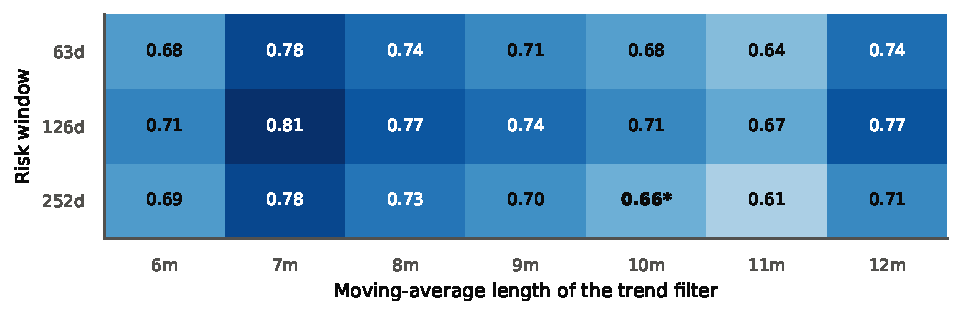
\includegraphics[width=\textwidth]{figures/fig_sensitivity.pdf}\resmark{fig_sensitivity}
\end{figure}


\section{Machine-learning extension}
\textbf{Question and model.} We tested whether machine learning detects stressed markets better than the trend
filter. A two-state Gaussian hidden Markov model (HMM; \citealp{hamilton1989,rabiner1989}) learns a calm and a
turbulent regime from daily S\&P 500 returns and volatility since \res{hmm_data_start}; regime models of this kind are
established in asset allocation \citep{ang2002,nystrup2018}. To avoid look-ahead, the model is re-estimated every
December on past data only, and each month uses the \emph{filtered} probability of the turbulent state given data up
to that day. Smoothed or Viterbi state paths, which use future data and make many published HMM backtests look better
than they are, are never used for decisions. In risk-off months the growth assets (SPY, EFA, VNQ, DBC) are halved.
A simple volatility rule serves as non-ML baseline. Before the first run we fixed all thresholds and three promotion
gates: Sharpe ratio at least that of the base strategy, a drawdown no deeper, and a better return in at least two of
the three stress periods.

\begin{table}[!htb]
\centering\small
\caption{Machine-learning variants, \res{sample_start}--\res{sample_end}, net of \res{cost_bps} per unit of turnover}\label{tab:ml}
\begin{tabularx}{\textwidth}{@{}Xrrrr@{}}
\toprule
\rowcolor{fmdark}\textcolor{white}{\textbf{Same months, net of costs}} & \textcolor{white}{\textbf{A: Trend}} & \textcolor{white}{\textbf{B: Vol.\ rule}} & \textcolor{white}{\textbf{C: HMM}} & \textcolor{white}{\textbf{D: Trend+HMM}} \\
CAGR (\% p.a.) & \resval{ml_a_cagr}{tab_ml}{4.6} & \resval{ml_b_cagr}{tab_ml}{5.3} & \resval{ml_c_cagr}{tab_ml}{4.9} & \resval{ml_d_cagr}{tab_ml}{4.2} \\
Volatility (\% p.a.) & \resval{ml_a_ann_vol}{tab_ml}{4.7} & \resval{ml_b_ann_vol}{tab_ml}{6.4} & \resval{ml_c_ann_vol}{tab_ml}{6.0} & \resval{ml_d_ann_vol}{tab_ml}{4.5} \\
Sharpe ratio & \resval{ml_a_sharpe}{tab_ml}{0.66} & \resval{ml_b_sharpe}{tab_ml}{0.61} & \resval{ml_c_sharpe}{tab_ml}{0.58} & \resval{ml_d_sharpe}{tab_ml}{0.61} \\
Maximum drawdown (\%) & \resval{ml_a_max_dd}{tab_ml}{$-$5.7} & \resval{ml_b_max_dd}{tab_ml}{$-$15.7} & \resval{ml_c_max_dd}{tab_ml}{$-$12.2} & \resval{ml_d_max_dd}{tab_ml}{$-$5.3} \\
Beta vs S\&P 500 & \resval{tab_ml}{tab_ml}{0.10} & \resval{tab_ml}{tab_ml}{0.22} & \resval{tab_ml}{tab_ml}{0.19} & \resval{tab_ml}{tab_ml}{0.07} \\
Turnover (\% p.a.) & \resval{ml_a_turnover}{tab_ml}{215.7} & \resval{ml_b_turnover}{tab_ml}{77.8} & \resval{ml_c_turnover}{tab_ml}{85.2} & \resval{ml_d_turnover}{tab_ml}{226.5} \\
Average T-bill weight (\%) & \resval{tab_ml}{tab_ml}{31.6} & \resval{tab_ml}{tab_ml}{3.6} & \resval{tab_ml}{tab_ml}{6.6} & \resval{tab_ml}{tab_ml}{34.5} \\
Stress periods better than A & -- & \resval{ml_b_stresswins}{tab_ml}{0 of 3} & \resval{ml_c_stresswins}{tab_ml}{0 of 3} & \resval{ml_d_stresswins}{tab_ml}{2 of 3} \\
Promotion gates passed & -- & \resval{ml_b_verdict}{tab_ml}{no} & \resval{ml_c_verdict}{tab_ml}{no} & \resval{ml_d_verdict}{tab_ml}{no} \\
\bottomrule
\end{tabularx}
\resmark{tab_ml}
\end{table}

\textbf{Result.} The HMM flags \res{ml_recall_hmm} of the \res{ml_n_stress} stress months (S\&P 500 down more than
\res{ml_stress_threshold} in the next month), more than the trend signal (\res{ml_recall_trend}). But only \res{ml_precision_hmm} of its
alarms are followed by such a fall, and it is risk-off in \res{ml_riskoff_hmm} of all months. Replacing the trend filter
(C) lowers the Sharpe ratio to \res{ml_c_sharpe} and deepens the drawdown to \res{ml_c_max_dd}, because the trend filter
also exits Treasuries when they fall. As an overlay (D) the HMM trims the drawdown to \res{ml_d_max_dd} but costs return
through extra cash and turnover (Sharpe \res{ml_d_sharpe}). No variant passes the gates (C \res{ml_c_verdict},
D \res{ml_d_verdict}); the result is the same for every random start and similar with three states
(\res{ml_3state_sharpe}). For our client this is a useful negative result: better crisis \emph{prediction} is not
automatically a better \emph{portfolio}, so the prospectus strategy stays rule-based.


\section{Interactive app}
The interactive app at \url{\appurl} runs the same code as the notebook: its calculation module is generated from the
notebook's cells. Users can switch the trend filter off, change the moving-average length, the risk window, the weighting
scheme (risk parity, Hierarchical Risk Parity, inverse volatility, equal weights), trading costs, the benchmark, the start
year and the asset classes held, and immediately see cumulative performance, drawdowns, weights and all measures against
the benchmark. A \emph{machine-learning and robustness lab} switches the variants of Section~9 on and off (Ledoit-Wolf
covariance, the averaged trend signal, the HMM or volatility overlay, leverage) and shows the verdict of the pre-registered
gates; the classifier and FinBERT variants, too heavy to recompute, are shown from the notebook's exported monthly returns.
With default settings the app reproduces Table~\ref{tab:performance}. Source code, dependencies and run instructions:
\url{\repourl}.


\section*{References}
{\footnotesize
\renewcommand{\bibsection}{}
\bibliographystyle{plainnat}
\setlength{\bibsep}{0pt}
\setlength{\columnsep}{14pt}
\begin{multicols}{2}
\bibliography{references}
\end{multicols}
}

\end{document}
